\documentclass[12pt, oneside, a4paper]{book}

% ----------------------------------------------------------------------------
% Preamble
% ----------------------------------------------------------------------------

% Package to manage page layout
\usepackage[a4paper, top=25.4mm, bottom=25.4mm, right=25.4mm, left=40mm]{geometry}

% Line spacing: single=1 one-and-a-half=1.3 double=1.6
\linespread{1.3}

\usepackage{adjustbox}

% Package to manage appendix
\usepackage[toc]{appendix}

% Package to insert empty lines between paragraphs
\usepackage[parfill]{parskip}

% Package to manage headers and footers
\usepackage{fancyhdr}

% define two header-footer styles
% 'normal' for most pages
\fancypagestyle{normal}{
\fancyhf{}
\fancyhead[L]{\slshape \leftmark} %chapter
\fancyhead[R]{\thepage} %footer
\renewcommand{\headrulewidth}{1pt}
}
% 'chapterstyle' for start of chapters (no chapter in header)
\fancypagestyle{chapterstyle}{
    \fancyhf{}
    \fancyhead[R]{\thepage}
    \renewcommand{\headrulewidth}{0pt}% Line at the header invisible
}

% Package to automatically change headerfooter style at start of chapters
\usepackage{etoolbox}
\patchcmd{\chapter}{\thispagestyle{plain}}{\thispagestyle{chapterstyle}}{}{}

% Package to get hyperrlinks
\usepackage{hyperref}

% For code illustration
\usepackage{listing}
\usepackage{minted}

% colouring of code
\usepackage{xcolor}
\definecolor{LightGray}{gray}{0.95}
\definecolor{LightBlue}{rgb}{0.98,0.98,0.92}

\usemintedstyle{pastie}

%New colors defined below
\definecolor{codegreen}{rgb}{0,0.6,0}
\definecolor{codegray}{rgb}{0.5,0.5,0.5}
\definecolor{codepurple}{rgb}{0.58,0,0.82}
\definecolor{backcolour}{rgb}{0.95,0.95,0.92}

% Mathematics packages
\usepackage{amsmath}
\usepackage{amssymb}
\usepackage{mathtools}

% A package to include graphics files (jpg, png, eps, pdf etc...)
\usepackage{graphicx}
\graphicspath{ {../img/} }

% A package that gives more control for bibliographies than the default
\usepackage[backend=biber, backref=true, firstinits=true, url=true, isbn=true]{biblatex}
\addbibresource{bibliography.bib}

% Package for mutli column list
\usepackage{multicol}

% Package to add features for tables
\usepackage{multirow}
\usepackage{booktabs}
\setlength{\heavyrulewidth}{1.5pt}
\setlength{\abovetopsep}{4pt}

% Package to allow sub-figures
\usepackage{subcaption}


% A package to generate latin. You do not need this: I am just using it to get
% random text.
\usepackage{lipsum}

% A package for vector graphics
\usepackage{tikz}
\usetikzlibrary{graphs,graphs.standard}
\usetikzlibrary{matrix, calc}

% A package for algorithms
\usepackage{algorithm}
\usepackage[noend]{algpseudocode}

\makeatletter
\def\BState{\State\hskip-\ALG@thistlm}
\makeatother

% ----------------------------------------------------------------------------
% The actual report
% ----------------------------------------------------------------------------

\begin{document}

\newgeometry{a4paper, top=25.4mm, bottom=25.4mm, right=25.4mm, left=25.4mm}
\input{title}
\restoregeometry

\frontmatter
\pagestyle{chapterstyle} %set header-footer style for front matter
\chapter{Executive Summary}
This dissertation investigates, the aspect of network topology, for the popular
Iterated Prisoner's Dilemma tournaments, a particular topic of  Game
Theory, and it is performed by taking advantage of the Axelrod-Python library.

This dissertation was completed during the taught program of Operational Research
and Applies Statistics of Cardiff University, under the supervision of Dr Vince
Knight.

In the 1980s, a tournament for the game of Iterated Prisoners Dilemma, spawned to
life a new area of research for Game Theory. Various scientists, from different
research fields, have ever since contributed to this research with concepts
such as noise, altered set of rules, probabilistic endings, further strategies and etc.
In 1992 new aspect was introduced: tournaments on different topologies.
In this new topology, players will not interact will all the player, but instead
were allocated on to networks and would interact with all the players to whom they have a
connection. This dissertation has focused on understanding the aspects of
this new topology, by using network analysis.

Throughout this work there are two underlying strands: data generation (carried
out by running a large number of tournaments) and data analysis.
Two experiments have been conducted. The first experiment, has been an initial
experiment trying to understand the spatial structure and find proper measures
of performance accuracy. Simple networks have been used for the tournament
topologies. Particularly, there have been three types of tournaments.
The first, a spatial tournament with a periodic lattice topology, the
second a spatial tournament of a cyclic topology and a round robin tournament.

The second experiment, was held to understand in depth the affects of the
topology. Using three different type of methods, spatial tournament have been
played. and afterwards their results have been studied. The median normalized
rank have been chosen as the performance measure.

Even so, out of all 132 strategies that have been given to us from the Alexrod-Python
library, none managed to outperform the rest. Thus in the final chapter, a
strategy has been trained,

From the mathematical aspects Graph Theory, Machine Learning, Clustering and
Genetic algorithm have been explored, to answer to the questions that this
dissertation have set.

\chapter{Acknowledgements}
There have been various people that work in Cardiff University that I would
like to thank for their support during this intense year.


I would like to thank all the lecturers of Cardiff University that taught on
the MSc taught program, for enlightening me and my collegues through their teaching.
Also for their continuous support and guidance through the year.
I would like to extend a special thank you to Mrs Joanna Emery for making this
entire year possible for me. Finally, I would like to express my sincere gratitude
to my academic supervisor Dr Vince Knight, for his support, advice and constant
ideas. To whom I lied once during this dissertation; yes the tables were being
overwritten.


\tableofcontents
\listoffigures
\listoftables
\chapter{Summary}

Ever since 1980, when a simple Iterated Prisoner's Dilemma(IPD) computer
tournament was conducted with 13 participants, new IPD tournaments have been run
and new strategies are constantly developed. This has inspired scientists to develop
an open source Python library, for reproducing all the research done on the topic
of the IPD. The library is called Axelrod-Python library, and furthermore it continuously holds
an IPD tournament with the, currently 132, implemented strategies.

The Axelrod-Python library, has become a powerful tool for the Game theoretic community.
Even so, up until this dissertation it lacked the ability to create tournaments on a variety of
topologies (a part from the basic round robin).
During this dissertation, the ability to
produce tournaments of a network topology; spatial tournament, was materialized.
Instantly, new questions were raised;such as what are the effects of the topology?

For addressing this questions the following approach was chosen. Identify the
effects of the topology on the performance of the strategies of the library and
does any of this strategies perform well in different tournaments of different
topologies. Thus throughly the research experiments have been conducted. In these
experiments simple and complex networks respectively have been used as topologies
to generate a number of spatial tournaments. Furthermore, non of the
Axelrod-Python library strategies was characterized as an overall satisfactory
strategy through the experiments. For this reason a variety of new strategies have
been trained using a genetic algorithm.


\mainmatter
\pagestyle{normal} %set header-footer style rest of report


\chapter{Introduction}
Game theory is a set of analytical tools and solution concepts, which provide
explanatory and predicting power in interactive decision situations, when the
aims, goals and preferences of the participating players are potentially in
conflict, Szabo and Fath (2007) \cite{Szabo2007}. The Prisoner's Dilemma(PD) is a well
known example in Game Theory and in recent years has become the gold standard of
understanding evolution of co-operative behavior \cite{Lorberbaum1994}.
Thus, it has been a topic of focus in various fields, such as biology,
sociology, ecology and psychology.

In the example of the Prisoner's Dilemma(PD) two criminals have been arrested
and interrogated, with no way of communicating, by the police. They are given
only two choices, to either cooperate with each other or to defect.
Consider that the prisoners would be put back in their cells and would be asked
the same question tomorrow. Furthermore, let this happen repeatably. This is
referred to as the Iterated Prisoner's Dilemma(IPD) an example that has been a
rich source of research material since the 1950s but has earned much interest in
the 1980s due to the work done by the political scientist Robert Axelrod
\cite{Axelrod1980a, Axelrod1980b, Axelrod1981}.

In 1980, Axelrod held the first ever IPD computer tournaments \cite{Axelrod1980a,
Axelrod1980b}, he invited
academia from various fields to submit their strategies in computer code. The
tournaments were of a round robin topology, the first competition included thirteen
strategies, while the second one sixty-four. In both tournaments the strategy Tit
for Tat was announced the winner and for many years it was considered to be the
most successful strategy. Tit for Tat is a deterministic strategy that will
always cooperate in the first round and afterwards it copies the opponents last
move.

A large volume of literature emerged on the topic following this, including some
criticism about these initial tournaments. Scientists questioned whether the
conditions that the first tournament took place favored Tit for Tat~\cite{RePEc:mtp:titles:0262023636}.
An argument was that the initial tournaments though they included
a 1\% chance of players misunderstanding their opponent's move in any round
,they did not examine noise. Noise is the probability
that the player will submit the wrong move. David and Vivian Kraines \cite{kraines-1989a}
stated that, Tit for Tat performed rather poorly when noise was introduced in the tournament.
Another aspect, is the payoff matrix, which according to Kretz \cite{Kretz2011},
effects the results.

Furthermore, another aspect needed to be taken into account is the network
topology underlying the tournament. In 1992 Nowak's and May's paper \cite{Nowak1992},
spatial tournaments are introduced. In their version of a spatial tournament,
the players are placed on an two-dimensional spatial array and allowed to play a
game with only the immediate neighbors. Thus, squares that are adjoint.
An example of this is shown in Figure~\ref{fig:nowak-example}.

\begin{figure}[!hbtp]
	\centering
		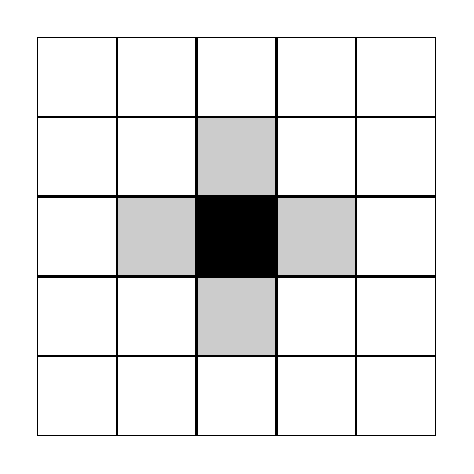
\begin{tikzpicture}

\matrix (input) [matrix of nodes,
                nodes={rectangle, draw=black, minimum size=1cm}] at (0,0)
{
|[fill=white!20]| & |[fill=white]|     & |[fill=white]|      &    |[fill=white]|     &    |[fill=white]|    \\
|[fill=white]| & |[fill=white]|     & |[fill=black!20]|   &    |[fill=white]|     &    |[fill=white]|    \\
|[fill=white]| & |[fill=black!20]|  & |[fill=black]|      &    |[fill=black!20]|  &    |[fill=white]|    \\
|[fill=white]| & |[fill=white]|     & |[fill=black!20]|      &    |[fill=white]|     &    |[fill=white]|    \\
|[fill=white]| & |[fill=white]|     & |[fill=white]|      &    |[fill=white]|     &    |[fill=white]|    \\
};
%\node [draw] at (input.south) {};

\end{tikzpicture}

		\caption{Topology of Nowak's tournament}
  \label{fig:nowak-example}
\end{figure}

Their tournament considered the PD and the players could only defect or
cooperate.  They provided proof that cooperative behavior can emerge from a PD
tournament in spatial topology. Many works on the IPD and spatial tournament
were held due to their original paper. Such as \cite{Grujic2014, Nowak1993,
Maciver1992, Nowak1992, Brauchli1999, Meng2015, Lindgren1994}.
These tournaments use either the PD or IPD and simple to complex strategies.

One can argue that the real life interactions are better represented by spatial
tournament because in real life not all players interact with all opponents.
Additionally, an interesting aspect of the spatial topology are the results
compared to those of a round robin tournament. This dissertation will be focusing on
reproducing a spatial tournament with some of the most successful strategies of
various tournaments that have been held.

For replicating the spatial topology, various graphs have been used, compared to
other woks which have used only lattices. Graphs such as, cyclic,
small world, random and complete. The affects of the topology on the
effectiveness of these strategies, has been studied. Followed by the attempt to
use a genetic algorithm to train a strategy that performs well in any given
topology.

\section{The Prisoner's Dilemma}
The PD was originally formulated in Merril \cite{Flood1958},
who were working on the Flood-Desher Experiment at the RAND cooperation in 1950.
Later in 1950, the mathematician Albert W. Tucker presented the first formal
representation of the PD, titled  A Two-Person Dilemma in a seminar at
Stanford University \cite{GassAssad2005}.

A description of the PD, found in \cite{Li2011} is as follows:
There are two players that simultaneously have to decide to whether Cooperate (C)
or Defect (D) with each other, without exchanging information.

\begin{itemize}
  \item If both players choose to cooperate they will both receive a reward (\(R\))
  \item If a player defects and the other cooperates then the defector receives
  a temptation payoff (\(T\)) and the cooperator a sucker payoff (\(S\))
  \item If both players defect they will both receive a penalty (\(P\))
\end{itemize}

Figure~\ref{fig:pd_payoff} illustrates the payoffs matrix.

\begin{figure}[h!]
    \centering
    \includegraphics[scale=0.45]{chapter-one/pd_payoff.jpg}
    \caption{The payoff matrix for the Prisoners Dilemma}
    \label{fig:pd_payoff}
\end{figure}

Taking into account the assumptions that both players are rational
and that there is no way of communication between them. No matter what the choice
of the other players,  defecting will always be the dominant choice as it yields
a higher payoff than cooperation.
Thus, a pure Nash Equilibrium exists when both players defect. Even though, both
players would do better if they were to cooperate; creating the dilemma.

Furthermore, for this to hold there are some extra assumptions for the
relationship of the four outcomes. The \(T\) temptation to defect has to offer the
highest payoff to a player and the lowest the player could achieve has to be the sucker's
payoff \(S\).
Likewise, the reward for mutual cooperation should exceed that of mutual
defection \(P\). Thus the next condition is~\ref{firstassum}:

\begin{equation}\label{firstassum}
 T > R > P > S
\end{equation}

Moreover, it is assumed that the average of \(T\) and \(S\) is less than the reward for
mutual cooperation~\ref{secondassum} :

\begin{equation}\label{secondassum}
    R > (T+S)/2
\end{equation}

Same conditions such as rationality, no communication and (~\ref{firstassum}),
(~\ref{secondassum}),
apply for the IPD. An IPD is nothing more than a PD were
the players interact for an infinite number of times.

\section{Problem Description}
Axelrod's tournaments set a seed for generations of tournaments in the
Prisoner's Dilemma using computer modeling. Research has shown that by altering the
environment of a tournament the effectiveness of some strategies can change
radically. An aspect that has been investigated as to how the tournament results
can bee affected was the topology. Nowak and May \cite{Nowak1992} introduced the spatial topology
only to set yet another seed in the PD tournaments. Even so, spatial topology
still has not been fully explored with only a small number of papers focusing on
this specific topology.  A goal of this dissertation is to understand the
current state of the art in spatial prisoner’s dilemma tournaments.

As described in \cite{MacLane1971} the contemporary world is full of networks. That
is one of the main reasons this dissertation will be focusing on such topology.
Work done at this point consider spatial topology to be that of a square lattice
were each edge represents a player which interacting/playing with only his
neighbors in their von Neuman or Moore's neighborhood. A von Neuman neighborhood
comprises the four cells orthogonally surrounding a central cell where the
Moore's neighborhood eight cells. As shown in Figure~\ref{fig:neighborhood}.

\begin{figure}[!hbtp]
	\centering
	\begin{subfigure}[h]{0.45\textwidth}
		\centering
		\input{chapters/Neuman.tex}
		\caption{von Neuman's neighborhood}
	\end{subfigure}
	\hfill
	\begin{subfigure}[h]{0.52\textwidth}\centering
		\centering
		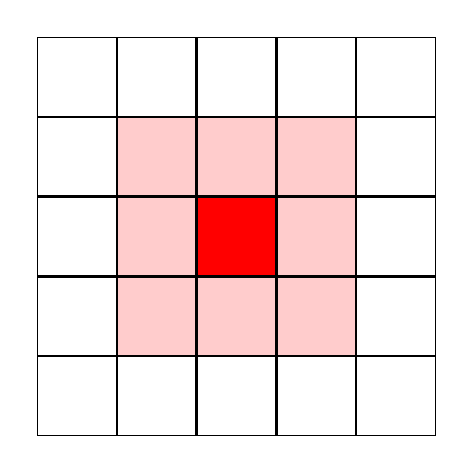
\begin{tikzpicture}

	\matrix (input) [matrix of nodes,
	nodes={rectangle, draw=black, minimum size=1cm}] at (0,0)
	{
		|[fill=white!20]| & |[fill=white]|      & |[fill=white]|      &    |[fill=white]|      &    |[fill=white]|    \\
		|[fill=white]|    & |[fill=red!20]|     & |[fill=red!20]|     &    |[fill=red!20]|     &    |[fill=white]|    \\
		|[fill=white]|    & |[fill=red!20]|     & |[fill=red]|        &    |[fill=red!20]|     &    |[fill=white]|    \\
		|[fill=white]|    & |[fill=red!20]|     & |[fill=red!20]|     &    |[fill=red!20]|     &    |[fill=white]|    \\
		|[fill=white]|    & |[fill=white]|      & |[fill=white]|      &    |[fill=white]|      &    |[fill=white]|    \\
	};
	%\node [draw] at (input.south) {};

\end{tikzpicture}

		\caption{Moore's neighborhood}
	\end{subfigure}
  \caption{Possible neighborhoods (a) A von Neuman's neighborhood where each node has four neighbors
  (b) A Moore's neighborhood where each node has eight neighbors}
  \label{fig:neighborhood}
\end{figure}

Some further work address the spatial topology in a variate of graphs
\cite{Dresher1992a, Szabo2007, Lutz2013, Meng2015}.
This dissertation will also follow this approach. Szabo and Fath dealt with
numerous graphs such as, lattices, small- world, scale free graphs and evolving
networks. Here a spatial topology is considered any given network where the
players are the nodes and only play other nodes that are linked to by
an edge.

Another disadvantage of the aforementioned work is that it lacked in terms of
best practice of reproducibility \cite{Axelrod1980a,Axelrod1980b,Stephens2002,Chong2004,Stewart2013}.
Due the work done by the Axelrod library \cite{axelrodproject} in the following research
the experiments are easily reproduced. As the library allows to produce an IPD
tournament and chose between 132 strategies already given by the library.
Code written for the purpose of this dissertation has been contributed to the
library: see \url{https://github.com/Axelrod-Python}.

\section{Analysis Tools}
Due to the high computational cost of the analysis considered, Cardiff
University's super computer, Raven, is used~\cite{raven}. All the scripts and pbs
file, for producing data with Raven can be found on can be found on github:
\url{https://github.com/Nikoleta-v3/jobs}. Furthermore, all data produced for
this work is archived using zenodo and can be readily downloaded. Details are
available in Appendix~\ref{append:data}.

For the data analysis the following libraries have been used:

\begin{multicols}{2}
	\begin{itemize}
		\item Numpy 1.11.1~\cite{numpy}
		\item Pandas 0.18.1~\cite{pandas}
		\item Matplotlib 1.5.1~\cite{matplot}
		\item Scipy: 0.18.0~\cite{scipy}
		\item Networkx 1.11~\cite{networkx}
    \item Scikit learn 0.17.1~\cite{scikit}
	\end{itemize}
\end{multicols}

\section{Structure of Dissertation}
This dissertation is organized into 6 Chapters. Following this introduction:
\begin{itemize}
  \item In~\autoref{chap:Two}, as well as introducing basic graph theory, all
        previous literature dedicated to the PD/IPD and tournaments that have
        been conducted, different topologies and evolution, have been reviewed
  \item In~\autoref{chap:Three} the main software contribution of this thesis is
        described: adding topologies to the Axelrod-Python software package.
        Some initial experiments and investigations are also carried out
  \item In~\autoref{chap:Four} a more in depth analysis in the topologies affects
				and the strategies performance is studied, by using various complex
				networks as the spatial tournaments topology
  \item In~\autoref{chap:Five} using a sophisticated evolutionary algorithm a
				new strategy is trained following the work conducted by Professor M Jones
				for his currently wining strategy EvolvedLookerUp
  \item In~\autoref{chap:Six} the results of this dissertation, as well as some
				further ideas for research are presented
\end{itemize}

\chapter{Literature Review}

Following the initial work done by Axelrod, there are many other papers that
have tried to tackle the PD and make their conclusions on cooperation in
both theoretical and real life behavior. In this chapter we review some of this
work done in the IPD competitions, in spatial and evolutionary game theory.

\section{Tournaments}

In order to get a understanding of how to play the game of the Prisoner's Dilemma
better, Robert Axelrod held a tournament back in 1980. He invited a number of
well-known game theorists to submit strategies for a computer tournament.
Each strategy has to specify whether to cooperate or defect based on the
history \footnote{The previous moves made by a player.} of both players.
Strategies played again each other as well as a Random strategy, that would
randomly choose between C and D and with its own twin. The tournament was of
round robin and all entries new the exact length (200 moves) of each game.
Fourteen strategies were submitted and by the end Tit for Tat was announced the
winner. Surprisingly in the second tournament held where 64 strategies
competed and all they writes had full knowledge of what have happened in the
first tournament, Tit for Tat managed to get first place again.\parencite{Axelrod1980a}

Tit for Tat is a deterministic strategy that will always cooperate in the first
round and afterwards it copies the opponents last move. Surprisingly in the
second tournament held by Axelrod \parencite{Axelrod1980a} where 64 strategies
competed and all they writes had full knowledge of what have happened in the
first tournament, Tit for Tat managed to get first place again.
As explained by Axelrod \parencite{Axelrod1980b}, Tit for Tat, a simple strategy was able to
win the rest of sophisticated and more complex strategies based on three specific
characteristics of the strategy:

\begin{itemize}
  \item Niceness:  A strategy is categorized as nice if it was not the
                    first to defect, or at least, it will not do this until
                    the last few moves.
  \item Forgiveness: The propensity to cooperate in the moves after the
                     opponent defected.
  \item Clarity: After opponents identified that they were playing Tit for Tat
                 choose to cooperate for the rest of the game.
\end{itemize}

The first tournaments were an innovation in combining computer modeling and Game
Theory and in providing insights in the behavior emerging from simple dynamics.
Moreover, Axelrod was the first to speak about niceness, forgiveness and gave an
illustration that cooperation can be a victorious and advantageous strategy.

There have been other tournaments, based off of Axelrod’s, exploring different
environments and submitting new strategies. In 1991 Bendor, Kramer and Stout
introduced noise to the IPD. Where noisy randomly flip the choice made by a strategy.
Kerts 2011 conducted a tournament where the payoff matrix was altered though
satisfying the conditions (1.1), (1.2) . In 1992, Nowak and May reproduced the first
tournament with a spatial topology. Furthermore, some review tournaments are
listed below :

% Do you think is a good idea to add a table with tournaments ?

\begin{table}[h]
\centering
\caption{An example table using the `booktabs' package}
\label{fig:exampletable}
\begin{tabular}{cccccccccc}
\toprule
& \multicolumn{3}{c}{\textbf{ABC}} & \multicolumn{3}{c}{\textbf{ABC}} & \multicolumn{3}{c}{\textbf{ABC}} \\
\cmidrule(lr){2-4}\cmidrule(lr){5-7}\cmidrule(lr){8-10}
\textbf{Example}      & \textbf{A}       & \textbf{B}       & \textbf{C}      & \textbf{A}           & \textbf{B}           & \textbf{C}          & \textbf{A}           & \textbf{B}           & \textbf{C}          \\
\cmidrule(lr){1-1}\cmidrule(lr){2-4}\cmidrule(lr){5-7}\cmidrule(lr){8-10}
0         & 1234      & 1234     & 1234     & 1234          & 1234         & 1234         & 1234        & 1234         & 1234         \\
1         & 1234      & 1234     & 1234     & 1234          & 1234         & 1234         & 1234        & 1234         & 1234         \\
2         & 1234      & 1234     & 1234     & 1234          & 1234         & 1234         & 1234        & 1234         & 1234        \\
3         & 1234      & 1234     & 1234     & 1234          & 1234         & 1234         & 1234        & 1234         & 1234         \\ \bottomrule
\end{tabular}
\end{table}

\section{Spatial Structure Tournaments}

A research was spawn in 1992 as to how the Prisoner's Dilemma could shade some
insight into physics and biology. Where they believed exist potential dynamics
of spatially extended systems. Their tournament was a simple and purely
deterministic spatial version of the PD in a two dimensional lattice. With
players having no memory of the previous rounds and no strategical elaboration.
Thus, the players could either always cooperate or defect. The local winner of
each generation would win a territory. His neighbors would follow his strategy.
This  allowed them generate spatial chaotic patterns, which patterns depended
on the payoff of Temptation. Nowak and May concluded that co-operational
behavior is possible in the PD by using a spatial topology.

Similarly, in \parencite{Lindgren1994} players were allowed to have
memory and therefore added complex strategies to the tournament such as Tit for
Tat and  Anti Tit for Tat. This was followed  by the work of
\parencite{Brauchli1999} which introduced even more
complex strategies.

Spatial topology has been defined most scholars have as a square lattice where
the nodes - players only interact with their neighborhoods.Including connections
between four or eight nearest neighbor sites, Neuman's or Moore's, according to
Figure~\ref{fig:neighborhood}. A square lattice  is a graph and one could argue
that a round robin tournament itself is a complete graph. But in the above papers
none author a spatial structure as graph, expect from \parencite{Meng2015} where
they defined it as a network.

Meng et all, was an interesting approach. They presented a new spatial prisoner's
dilemma game model in which the neighborhood size was increased onto two
two interdependent lattices. They implement the utility by integrating the payoff
correlations between two lattices. A player would mimic a random player in his next
move, base on a function that consider the utility of the player. It was characterized
as a most realistic scenario.

Real life interactions are more likely to be like any given graph depending on
the industry than a complete graph. Fatha et all, have considered a numerous of graphs,
such as :
\begin{itemize}
  \item Lattice, the interaction network is defined by the sites of a lattice.
   the distance between a pair does not exceed a given value.
   The most frequently used structure is the square lattice with von Neumann
   neighborhood and Moore neighborhood.
  \item Small word, a graph that is created from a square lattice by randomly
   rewiring a fraction of connections in a way that conserve the degree for
   each site.
  \item Scale-free graphs, a network that has a power-law degree distribution, regardless of
   any other structure.
  \item Evolving networks, networks that change as a function of time.
\end{itemize}

The major theme of their review was how the graph structure of interactions could
modify long term behavioral patterns emerging in evolutionary games.
These graphs compose only a small fraction of graphs that exist. In this
dissertation we will consider a list of graphs.
 %add list when i actually know

\section{Axelrod Python Library}

The Axelrod library (.ref) is an open source Python package that allows for
reproducible game theoretic research into the Iterated Prisoner's Dilemma[url].
For many of the tournaments aforementioned the original source code is almost never
available and in no cases is the available code well-documented, easily modified
or released with significant test suites. Due to that reproducing the results
has not been an easy task.

However, Axelrod library manages to provide such a resource, with facilities for
the design of new strategies and interactions between them, as well as
conducting tournaments and ecological simulations for populations of strategies.

Strategies are implemented as classes which have a single method, strategy().
It only takes one argument, which is the opponent's previous moves and returns
an action. These actions can be either to cooperate C or to defect D. At thins
moment the Axelrod library consists of 131 strategies.Can be found in the Appendix.

Additionally, tournament are classes responsible for running a repetition of a
round robins. It achieves that by calling a match generator class which
returns all the single match parameters, such as turns, the game and the noise.
Axelrod has the capability to write out the results into a csv file and also out
put plots with the ranks of the strategies.

Furthermore, a basic tournament of 200 turns, 100 repetitions and the 131 strategies
that exist in the library is being produced continuously. The winner is called
PSO gambler and it is a look up strategy. It uses a lookup table with probability
numbers generated using a Particle Swarm Optimisation (PSO) algorithm.
Here are illustrated the results of the last tournament :

\begin{figure}[h]
\centering
    \begin{subfigure}[t]{0.55\textwidth}
    \centering
        \includegraphics[width=\linewidth]{axl.png}
    \caption{Ranked violin plot}
    \end{subfigure}
\hfill
    \begin{subfigure}[t]{0.50\textwidth}\centering
    \centering
        \includegraphics[width=\linewidth]{axl1.png}
    \caption{Payoffs}
    \end{subfigure}
~
\caption{Result Plots. (a) Ranked violin plot, the mean utility of each player.
(b) Payoffs, the pair wise utilities of each player.}
\label{fig:axelrodplots}
\end{figure}

Because is an open source library it makes it easy for us to contribute to it
make modifications needed for this dissertation.


% This section on the library can/will be rewritten. See comment in chapter 1
% about citation.

\chapter{Implementation of spatial tournaments}
\label{chap:Three}

\section{Introduction}
In this chapter we will discuss some initial experiments and their results.
These experiments will be performed using three chosen topologies and two
different sizes of tournaments. Emphasis will be given in the analysis of the
results and identification of strategies behaviors. In addition, the source code
committed to the Axelrod-Python library to implement the spatial topology will
be discussed. As well as two important aspects of developing
test driven development and version control.

\subsection{Code Discussion}

As analyzed in \autoref{chap:Two}, the Axelrod library uses a
\texttt{Tournament} class to run any given tournament. The \texttt{Tournament}
class itself calls upon another class the \texttt{Match Generator} which is
responsible for generating matches.
In the case of a standard round robin, there is a \texttt{RoundRobinTournament} class
and a \texttt{RoundRobinMatches} class that generates matche parameters for each 2 player
tuple. The parameters and the indices of the pair are used
by the \texttt{build\_single\_match} method. A generator that lives within the
match generator class.
For a round robin tournament the structure of the code is illustrated
in~\ref{fig:round_robin_structure}.


\begin{figure}
\centering
    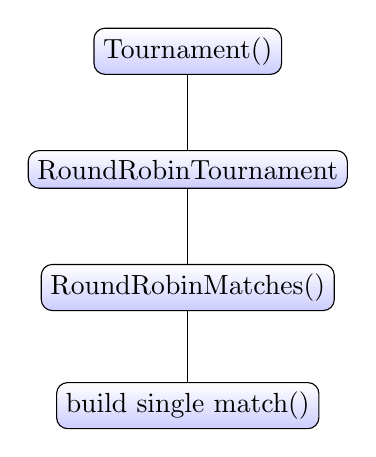
\begin{tikzpicture}[sibling distance=10em,
      every node/.style = {shape=rectangle, rounded corners,
        draw, align=center,
        top color=white, bottom color=blue!20}]]
      \node {Tournament()}
        child { node {RoundRobinTournament}
          child { node {RoundRobinMatches()}
            child { node {build single match()} } }
           };
    \end{tikzpicture}
  \caption{Code structure for a Round Robin tournament.}
  \label{fig:round_robin_structure}
\end{figure}

In order for to implement a Spatial topology tournament a similar approach is
needed. Firstly a new \texttt{Match Generator} class was written.  The
\texttt{SpatialMatches} is a class that generates spatially-structured matches.
In these matches, players interact only with their neighbors rather than the
entire population. According to \cite{Archdeacon1996} graphs can be represented
in many different ways, one of which is by lists of edges.  Due to a various
number of python packages that are used for graph manipulation, we want to keep
a more generalized representation of the edges. Thus they will be passed as a
list argument and \texttt{SpatialMatches} will only create matches between the
ending nodes of these edges. Finally the class \texttt{SpatialTournament} runs
the spatial tournament. A representation of the code structure now, that the
spatial tournaments have been added, can be seen in
Figure~\ref{fig:spatial_structure}

\begin{figure}
\centering
    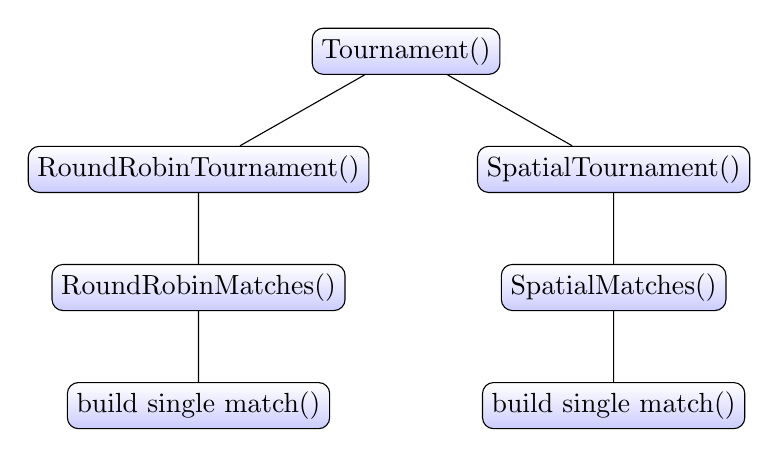
\begin{tikzpicture}[sibling distance=15em,
      every node/.style = {shape=rectangle, rounded corners,
        draw, align=center,
        top color=white, bottom color=blue!20}]]
      \node {Tournament()}
        child { node {RoundRobinTournament()}
          child { node {RoundRobinMatches()}
            child { node {build single match()} } }}
        child { node {SpatialTournament()}
          child { node {SpatialMatches()}
            child { node {build single match()} } }
           };
    \end{tikzpicture}
  \caption{Code structure for when Round Robin and Spatial tournaments are
           implemented.}
  \label{fig:spatial_structure}
\end{figure}

The Axelrod-Python library is a Test Driven Development (TDD) software.
All the components are automatically tested using a combination of unit,
property and integration tests (using \url{travis-ci.org}).
Once a new feature is added to the library, corresponding test must also be
written. The test are used to ensure compatibility and ensure that we get the
expected results. In~\cite{Developer} Percival explains from his personal
experiences the importance of TDD and having tests for every single line of code.
For the spatial tournament
new unit test have been added. Unit tests are used to invoke a unit of work and
check that the behavior is expected. A unit of work can be any single logical
functional use in the system. In summary, unit tests help to write clean and bug
free code~\cite{Developer}. The unit tests for the \texttt{SpatialTournament} can
be found below ~\ref{lst:test_spatial_tournament}.

\begin{listing}[H]
\usemintedstyle{tango}
\begin{minted}
[
frame=lines,
framesep=2mm,
baselinestretch=1.2,
bgcolor=LightBlue,
fontsize=\footnotesize,
linenos
]
{python}
class TestSpatialTournament(unittest.TestCase):

    @classmethod
    def setUpClass(cls):
        cls.game = axelrod.Game()
        cls.players = [s() for s in test_strategies]
        cls.test_name = 'test'
        cls.test_repetitions = test_repetitions
        cls.test_turns = test_turns
        cls.test_edges = test_edges

    def test_init(self):
        tournament = axelrod.SpatialTournament(
            name=self.test_name,
            players=self.players,
            game=self.game,
            turns=self.test_turns,
            edges=self.test_edges,
            noise=0.2)
        self.assertEqual(tournament.match_generator.edges, tournament.edges)
        self.assertEqual(len(tournament.players), len(test_strategies))
        self.assertEqual(tournament.game.score(('C', 'C')), (3, 3))
        self.assertEqual(tournament.turns, 100)
        self.assertEqual(tournament.repetitions, 10)
        self.assertEqual(tournament.name, 'test')
        self.assertTrue(tournament._with_morality)
        self.assertIsInstance(tournament._logger, logging.Logger)
        self.assertEqual(tournament.noise, 0.2)
        anonymous_tournament = axelrod.Tournament(players=self.players)
        self.assertEqual(anonymous_tournament.name, 'axelrod')
\end{minted}
\caption{Source code for TestSpatialTournament class, which is for testing the
         spatial tournaments.}
\label{lst:test_spatial_complete_tournament}
\end{listing}

\texttt{TestSpatialTournament()} it a simple class for a unittests written for
the spatial tournaments. In~\ref{lst:test_spatial_tournament}, whether
the values of the attributes were passed correctly is being tested. Also whether
the scores are as anticipated. In~\ref{lst:test_spatial_complete_tournament},
another test is shown. Here the results of a complete spatial tournament are
compared to those of a round robin one.

\begin{listing}[H]
\usemintedstyle{tango}
\begin{minted}
[
frame=lines,
framesep=2mm,
baselinestretch=1.2,
bgcolor=LightBlue,
fontsize=\footnotesize,
linenos
]
{python}
@given(strategies=strategy_lists(strategies=deterministic_strategies,
                                     min_size=2, max_size=2),
           turns=integers(min_value=1, max_value=20))
    def test_complete_tournament(self, strategies, turns):
        """
        A test to check that a spatial tournament on the complete multigraph
        gives the same results as the round robin.
        """
        players = [s() for s in strategies]
        # edges
        edges=[]
        for i in range(0, len(players)) :
            for j in range(i, len(players)) :
                edges.append((i, j))
        # create a round robin tournament
        tournament = axelrod.Tournament(players, turns=turns)
        results = tournament.play()
        # create a complete spatial tournament
        spatial_tournament = axelrod.SpatialTournament(players, turns=turns,
                                                       edges=edges)
        spatial_results =  spatial_tournament.play()
        self.assertEqual(results.ranked_names, spatial_results.ranked_names)
        self.assertEqual(results.nplayers, spatial_results.nplayers)
        self.assertEqual(results.nrepetitions, spatial_results.nrepetitions)
        self.assertEqual(results.payoff_diffs_means,
                                         spatial_results.payoff_diffs_means)
        self.assertEqual(results.payoff_matrix,
                                              spatial_results.payoff_matrix)
        self.assertEqual(results.payoff_stddevs,
                                             spatial_results.payoff_stddevs)
        self.assertEqual(results.payoffs, spatial_results.payoffs)
        self.assertEqual(results.cooperating_rating,
                                         spatial_results.cooperating_rating)
        self.assertEqual(results.cooperation, spatial_results.cooperation)
        self.assertEqual(results.normalised_cooperation,
                                     spatial_results.normalised_cooperation)
        self.assertEqual(results.normalised_scores,
                                          spatial_results.normalised_scores)
        self.assertEqual(results.good_partner_matrix,
                                        spatial_results.good_partner_matrix)
        self.assertEqual(results.good_partner_rating,
                                        spatial_results.good_partner_rating)
\end{minted}
\caption{Source code for testing a complete spatial tournament.}
\label{lst:test_spatial_tournament}
\end{listing}

The source code for the spatial tournaments and the tests can be found
in the Axelrod-Python library. The library is available at
\url{https://github.com/Axelrod-Python},
which is a hosted git repository. This introduce us to another important aspect
of software development, the version control system (VCS). \cite{Developer} stated
that TDD and VS go hand in hand. VCS, is a tool that manages and tracks different
versions of software~\cite{Vogel2014}. Software code is expanding continuously,
thus it can be an enormous
complicated system. Lines of codes are deleted, implementing errors occur and
programmers forget. Thus, having the ability to go back to any given point can be
very important. Git is a specific powerful and famous VSC. It was
invented by Linus Torvalds and was span to to life in April 2005.

The Axelrod-Python library is a project which includes numerous contributors.
Any given addition to the
library has to be submitted by a pull request. Each submission is then
reviewed by the members. This applies to the spatial tournament as well.
In Figure~ conversation containing comments and corrections can be seen.

%  screenshots, you said screenshots. I am keeping the proof here.

%  add screenshots from home.

O.Campbell and M.Harper are the main contributors of the library, alongside V.Knight.
Their work, in company of other contributors included myself, had an impact on
the Game Theory society. The project involves various research topics of
the IPD, such as Noise tournaments, Probabilistic ending and Spatial tournaments.
Strategies from different works and authors and the capability
of reproducing any of these given tournaments. A publication was achieved earlier
in 2016~\cite{Knight2016}.

In the next section an overview and a summary of the initial experiments
performed is given.


\subsection{Experiment and the three topologies}

In this chapter three simple spatial topologies are considered, all with
deterministic neighborhood size. These will be used to begin to understand how
topology can affect the outcome of tournaments
and which strategies tend to perform well. The three topologies considered are
well represented in the literature \cite{?}:

\begin{itemize}
    \item A cyclic network: the neighbourhood size is 2. % include specific references
    \item A periodic lattice: the neighbourhood size is 4. % include specific references
    \item A complete graph: the neighbourhood size if \(N-1\) (where \(N\) is
        the number of total strategies. This corresponds to a round robin
        tournament. % References
\end{itemize}

Figure~\ref{fig:networks}, shows an example of all the aforementioned topologies.

\begin{figure}[h]  % http://drvinceknight.blogspot.co.uk/2013/12/explaining-floats-in-latex.html
\centering
    \begin{subfigure}[h]{0.45\textwidth}
    \centering
        \includegraphics[width=\linewidth]{cycle_network.png}
    \caption{Cyclic network.}
    \end{subfigure}
\hfill
    \begin{subfigure}[h]{0.52\textwidth}\centering
    \centering
        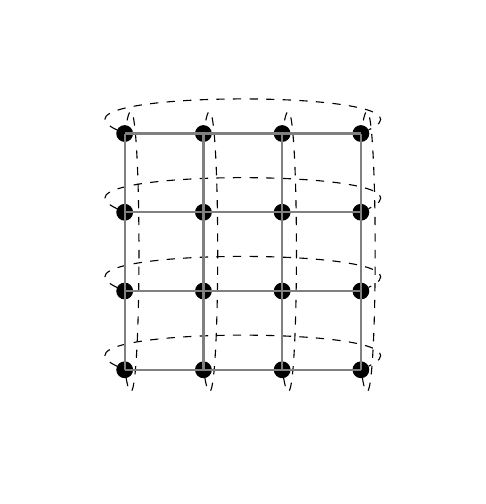
\begin{tikzpicture}

        % First column (tikz has the ability to use loops but I'm drawing it
        % this way so you see how.
        \node (00) [draw, circle, inner sep=2pt,fill] at (0, 0) {};
        \node (01) [draw, circle, inner sep=2pt,fill] at (0, 1) {};
        \node (02) [draw, circle, inner sep=2pt,fill] at (0, 2) {};
        \node (03) [draw, circle, inner sep=2pt,fill] at (0, 3) {};

        % Second column
        \node (10) [draw, circle, inner sep=2pt,fill] at (1, 0) {};
        \node (11) [draw, circle, inner sep=2pt,fill] at (1, 1) {};
        \node (12) [draw, circle, inner sep=2pt,fill] at (1, 2) {};
        \node (13) [draw, circle, inner sep=2pt,fill] at (1, 3) {};

        % Third column
        \node (20) [draw, circle, inner sep=2pt,fill] at (2, 0) {};
        \node (21) [draw, circle, inner sep=2pt,fill] at (2, 1) {};
        \node (22) [draw, circle, inner sep=2pt,fill] at (2, 2) {};
        \node (23) [draw, circle, inner sep=2pt,fill] at (2, 3) {};

        % Fourth column
        \node (30) [draw, circle, inner sep=2pt,fill] at (3, 0) {};
        \node (31) [draw, circle, inner sep=2pt,fill] at (3, 1) {};
        \node (32) [draw, circle, inner sep=2pt,fill] at (3, 2) {};
        \node (33) [draw, circle, inner sep=2pt,fill] at (3, 3) {};


        % I am drawing the periodic boundaries before the rest of the grid
        % so that they appear 'behind' the rest of the images.
        % Draw the period horizontal boundary
        \draw[dashed] (00) to[out=155,in=25 ] (30);
        \draw[dashed] (01) to[out=155,in=25 ] (31);
        \draw[dashed] (02) to[out=155,in=25 ] (32);
        \draw[dashed] (03) to[out=155,in=25 ] (33);

        % Draw the period vertical boundary
        \draw[dashed] (00) to[out=-80,in=80] (03);
        \draw[dashed] (10) to[out=-80,in=80] (13);
        \draw[dashed] (20) to[out=-80,in=80] (23);
        \draw[dashed] (30) to[out=-80,in=80] (33);

        % Draw a grid (this is a tikz shortcut)
        \draw[style=help lines,thick] (0,0) grid  (3,3);
\end{tikzpicture}

    \caption{Periodic lattice with degree 4 network.}
    \end{subfigure}
\hfill
    \begin{subfigure}[h]{0.52\textwidth}\centering
    \centering
        \includegraphics[width=\linewidth]{complete-network.png}
    \caption{A complete or round robin network.}
    \end{subfigure}
\caption{Network topologies.}
\label{fig:networks}
\end{figure}

For each topology, a fixed number of strategies out of the 132 of Axelrod-Python
library are chosen randomly. The number of strategies define the size of the
tournament. In the experiments the tournament size can be either five or fifty.

Subsequently, the strategies are allocated on the graph, based
on the topology, and they compete with their neighbors on a IPD tournament.
For the cyclic and lattice topology, once the first game is complete,
the strategies are randomly shuffled and allocated on the graph again. This aims
to ensure that their particular position on the network is taken in to account.
This shuffle is repeated 10 times. The selection of strategies is repeated 100 times
and each tournament of an IPD consists of 200 turns and 10 repetitions.
Listing~ illustrates these rules.

\begin{listing}[H]
\usemintedstyle{tango}
\begin{minted}
[
frame=lines,
framesep=2mm,
baselinestretch=1.2,
bgcolor=LightBlue,
fontsize=\footnotesize,
linenos
]
{python}

\end{minted}
\caption{Source code for TestSpatialTournament class, which is for testing the
         spatial tournaments.}
\label{lst:test_spatial_complete_tournament}
\end{listing}

% I think you should draw a picture of this or perhaps write some pseudo code
% (kind of like the things we've been writing on my whiteboard):
% http://tex.stackexchange.com/questions/163768/write-pseudo-code-in-latex

% seeds allow us
% reproduce the same players and tournaments.},
% You're going in to to many details here: the reader could potentially have no
% idea what Numpy is. If you write this out with pseudo code you can simply say
% that you're looping over seeds and then include some nice reference/comment
% about why you're doing that.

The Axelrod tournaments themselves make usage of match memory and CPU power and
by adding these additional rules to the tournaments was only increasing in usage.
For that reason all the tournaments and their results are runned in Raven.
Raven is the super computer of Cardiff University. All the scripts and pbs file, for
communicating with Raven, can be found on github :
\url{https://github.com/Nikoleta-v3}.

For the data preparations and analysis the following libraries have been used:
\begin{multicols}{2}
  \begin{itemize}
    \item Numpy 1.11.1:
    \item Pandas 0.18.1:
    \item Matplotlib 1.5.1:
    \item Statsmodels 0.6.1:
    \item Networkx 1.11:
  \end{itemize}
\end{multicols}

Furthermore, some simple functions for measures such as neighborhood scores
were written.

% I have to create a repository with all the files for the dissertation and clean
% thing up a little bit. Then I will add the new link here. and a message 'Like my page :D'

% Haha: good idea :) We'll also talk about using something like zenodo.org to
% 'freeze' your data. We should talk about this.

In the next section, an initial analysis of the experiments aforementioned
is held. Moving on in section~\ref{sub:effects} to a more intense analysis. The
concept of winning ratio and normalized average score are introduced. Finally,
summarizing the results in~\ref{sub:summary}, offering further avenues  of research.


\subsection{Initial Analysis}

For each of the tournament run, the following parameters are recorded:

\begin{multicols}{3}
  \begin{itemize}
    \item players list
    \item seed
    \item parameter
    \item player index
    \item player name
    \item cooperating ratio
    \item degree
    \item neighbors
    \item neighborhood size
    \item ranking
    \item scores
    \item normalized scores
    \item average score
    \item R
    \item P
    \item S
    \item T
    \item connectivity
    \item clustering
    \item cliques
    \item neighbors scores
    \item normalized neighbors score
    \item normalized average neighborhood score
  \end{itemize}
\end{multicols}

This section will describe the findings of a basic statistical analysis of these
records.

For the spatial tournaments, for both tournament sizes (5 and 50)
5Also, we have so far used the
% terminology that the complete graph is a spatial tournament (just a boring
% topology so this needs to be reworded to fit with that).
we achieved 1000 tournaments. Containing 100 different strategy sets, where each
the exists for 10 tournaments.

Moreover, for the cyclic experiment we can see in Table~\ref{sum-cicle}, that degree is
fixed at 2 and the payoffs are fixed to \(R=3, P=1, S=0, T=5\) for both
tournament sizes. For tournaments of size 5, the mean average score
is 2.45, with a minimum value of 0.0175 and a maximum value of 4.95. The
mean average score of the neighbors score is 980.95 with a standard deviation
of 219.87. Moreover the minimum value is set at 141.55 and the maximum at
1756.50. The mean average score does not seem to differ for size equal 5,
which is at 2.39. Though, in the experiment with a size of fifty a strategy
achieved a score of 0. Additionally the average score of the neighbors ranges
from 19.30 to 1884.5. Concerning the graph measures, as explained in [chapter 2],
clustering coefficient is zero and connectivity fixed to 2.
% Also I forget, but assuming you have described what these things mean in C2,
% you should remind the reader and just point them to C2.

% This table looks good BUT (IMPORTANT) Read these (and then improve all your
% tables)
% - http://www.howtotex.com/packages/improve-your-tables-with-booktabs/
% - https://www.inf.ethz.ch/personal/markusp/teaching/guides/guide-tables.pdf
%   (particularly the before and after slide)
\begin{table}[!hbtp]
\centering
\begin{adjustbox}{width=1\textwidth}
\small
\begin{tabular}{@{}|l|l|l|l|l|l|l|l|l|l|@{}}
\toprule
Cyclic & \multicolumn{3}{c|}{tournament size 5 and 50} & \multicolumn{3}{c|}{tournament size 5} & \multicolumn{3}{c|}{tournament size 50}                             \\\midrule

       & (R,P,S,T) & degree & connectivity & average score & average neighbors score & clustering & average score & average neighbors score & clustering \\\midrule
mean   & (3,1,0,5) & 2.0    & 2.0          & 2.45      & 980.95            & 0.00       & 2.39     & 957.23             & 0.00       \\\midrule
std    & (0,0,0,0) & 0.0    & 0.0          & 0.74      & 219.87             & 0.00       & 0.77    & 231.32              & 0.00       \\\midrule
min    & (3,1,0,5) & 2.0    & 2.0          & 0.01      & 141.55             & 0.00       & 0.00    & 19.30              & 0.00       \\\midrule
max    & (3,1,0,5) & 2.0    & 2.0          & 4.95     & 1756.50             & 0.00       & 5.00    & 1884.50             & 0.00       \\ \bottomrule
\end{tabular}
\end{adjustbox}
\caption{Summary table for topology circle.}
\label{sum-cicle}
\end{table}

For the lattice topologies a table that summarizes the data set is shown in Table
~\ref{sum-lattice}. For both size values the payoffs are the same (\(R=3, P=1, S=0, T=5\))
and the degree is fixed at 4. For size 5 the mean average score
varies between 0.018 and 4.97. The average score of the neighbors varies between
832.67 and 2895.42. Much higher than both the cyclic experiments achieved. This
is understood to be based on the fact that the number of neighbors is now doubled.
For size 5 the mean score is 0.57 and the mean average neighbor score 2.45.
The clustering coefficient is 1 and for size 50 is 0.5.
This shows that in the lattice example the strategies tend to create groups.
% What do you mean about 'groups'. I don't disagree, just curious.

\begin{table}[!hbtp]
\centering
\begin{adjustbox}{width=1\textwidth}
\small
\begin{tabular}{@{}|l|l|l|l|l|l|l|l|l|l|@{}}
\toprule
Lattice & \multicolumn{3}{c|}{tournament size 5 and 50} & \multicolumn{3}{c|}{tournament size 5} & \multicolumn{3}{c|}{tournament size 50}                            \\ \midrule
       & (R,P,S,T) & degree & connectivity & average score & average neighbors score & clustering & average score & average neighbors score & clustering \\ \midrule
mean   & (3,1,0,5) & 4.0    & 4.0          & 2.45      & 1958.56           & 1.0        & 2.39      & 1912.74             & 0.5        \\ \midrule
std    & (0,0,0,0) & 0.0    & 0.0          & 0.57      & 287.63            & 0.0        & 0.59      & 268.37              & 0.00       \\ \midrule
min    & (3,1,0,5) & 4.0    & 4.0          & 0.52      & 1059.77           & 1.0        & 0.01      & 832.67              & 0.5        \\ \midrule
max    & (3,1,0,5) & 4.0    & 4.0          & 4.24     & 2518.70            & 1.0        & 4.97      & 2895.42             & 0.5        \\ \bottomrule
\end{tabular}
\end{adjustbox}
\caption{Summary table for the lattice topology.}
\label{sum-lattice}
\end{table}

\newpage

Finally, for the round robin tournaments, 100 tournaments were performed for both
sizes. Parameters such as neighborhood size and neighbor's score
were not computed for the round robin topology. This is because all players
interact with each other thus there were not any additional information to be
gained. In Table~\ref{sum-rr}, the average score the strategies achieved
in this topology for both sizes is shown. In a tournament of size 50, the mean average
score is 2.39 with a standard deviation of 0.335.

\begin{table}[H]
\centering
\begin{tabular}{|l|l|l|}
\hline
Round Robin & \multicolumn{1}{c|}{tournament size 5} & \multicolumn{1}{c|}{tournament size 50} \\ \hline

            & average score            & average score             \\ \hline
mean        & 2.447105                 & 2.393220                  \\ \hline
std         & 0.576014                 & 0.335552                  \\ \hline
min         & 0.527500                 & 1.523673                  \\ \hline
max         & 4.245000                 & 3.339592                  \\ \hline
\end{tabular}
\caption{Summary table for round robin topology.}
\label{sum-rr}
\end{table}

In this section the structure of the source code for implementing the Spatial
Tournament, by adding to the Axelrod-Python library was analyzed. Furthermore,
now that the code is usable various experiments were conducted with different
topologies
and number of players participating in each tournament. An overview of the
data sets produced was done but now in the following sections
some more analysis on the results will be performed.

\newpage
\section{Analyzing the effect of the topologies}
\label{sub:analyzing_the_effect_of_the_topologies}

In the data all 132 strategies of Axelrod-Python library have participated at
least in one tournament. Not all strategies participated in an equal
number of tournaments.
Forcing the strategies to perform in a uniform number is
not an option because the random effect is needed for validation of the
results. But one could argue that by participating in a larger number of
tournaments, the probability of winning increases as well.
Thus, for a measure of
performance, instead of using the number of tournaments won, the analysis will
be using the ratio of wins in subsection~\ref{sub:winning-ratio}.
The winning ratio is defined as the number of tournaments a strategy was ranked
first divided by the number of tournaments the strategy competed in.
Additionally, the normalized average score each strategy
achieved will also be studied in subsection~\ref{sub:normalized_av_score}. Mainly to study
the variation, helping with conclusions on the performance of a strategy.
Lastly in subsection~\ref{sub:regression}, having all different
factors such as degree, neighbors, clustering, scores etc building a regression
model could point out effects on the results.


\subsection{Winning Ratio}
\label{sub:winning-ratio}

The winning rations for all three topologies for tournaments of size 5
are shown in Figure~\ref{fig:winning-five}. In the experiment where the
strategies compete on a cyclic 124 strategies out of the 132 have a
winning ration greater than zero. In other words 8 strategies won no
tournaments. These strategies are ALLCorALLD,
Tricky Cooperator, ThueMorseInverse, Hard Tit For 2 Tats, SolutionB5, cyclicr DDC,
Prober and BackStabber.
% Put these in a bullet point list or a table with a VERY brief description of
% what they do.
% I'm really surprised that BackStabber won no tournaments...
In the lattice topology as well, 8 strategies do not have
a non-zero winning ratio. Fortress4, Bully, Tricky Cooperator, Hard Go
By Majority: 5, 10 and 40. Also cyclicr DDC and ALLCorALLD have a similar
performance in this topology as well.
% Same comment about putting the strategies in a table.
In the round robin tournament various strategies  % How many?
ranked last, among them Fortress4 and the whole family of Hard Go By Majority.
% If the number is not stupid perhaps put them in a table also.

On the other hand the strategies with the highest winning ratio for each
topology are as follows:

\begin{itemize}
  \item Cyclic topology with a winning ratio of 0.56 ZD-GEN-2, followed by Punisher
        with 0.55
  \item Lattice topology with a ratio of 0.45 BackStabber and Meta Majority
        Memory one
  \item Round Robin topology with a winning ratio of 1 : Raider, Gradual, Limited
        Retaliate(0.05/20) and BackStabber.
        % See how well Backstabber does here and on the lattice...
        % I wonder what's going on... Interesting...
        % Will be good to get those line plot things.
\end{itemize}

In every topology the highest ranking strategy between the size five experiments
are different. Only BackStabber seems to be repeated, even so in the cyclic topology
 it had a winning ratio of zero. ALLCorALLD, did badly in all
three topologies.

When considering tournaments of size 50
no strategies have a zero ratio (in any topology).
% Give a little explanation for this: why do we think that is? Does this perhaps
% mean we need to run the size 5 strategies more? To get more diversity in the
% strategy sets? What do you think?
Figure~\ref{fig:winning-fifty}, illustrates the ratios
for each topology in ascending order. The strategies with the highest winning ratio
for each respective topologies are as follow :

\begin{itemize}
  \item cyclic topology with a winning ratio of 1.3 Raider
      % Winning ratio of 1.3? 1.3 > 1
  \item Lattice topology with a winning ratio of 1.3 Raider
  \item Round Robin topology with a winning ration of 0.833 EvolvedLookerUp
\end{itemize}

Unexpectedly, strategy Raider seems to have first place in both
the cyclic and the lattice topology. It achieved a winning ration of 1.3, 0.5
more than the strategy ranked second. Another surprise in the results is
that of the round robin topology. Where a large number of strategies have a
winning ratio
of zero. Only 14 strategy managed a ratio higher than zero. The strategy with
the highest one of all was EvolvedLookerUp.

Overall, in all six experiments the only strategy that seems to be repeatedly
have a high performance is
Raider. Compared to all the other strategies that outperformed the rest the seem
to be no similarity in their way of structure and play. Here we could use
a characterization to compare the strategies more efficiently. The winning ratio
seems to vary from zero to 1.3 and in the round robin topology many strategies
seem to get zero.
% winning ratio higher than 1?

% add plot
% The line plot yes? I think this will be 3 line plots, one for each comparison
% of topology. This will be very good to have.

\begin{figure}[!hbtp]
\centering
    \begin{subfigure}[t]{1\textwidth}
    \centering
        \includegraphics[width=\linewidth]{winners-cycle_five.pdf}
    \caption{Winning ration cycle s=5.}
    \end{subfigure}
\hfill
    \begin{subfigure}[t]{1\textwidth}\centering
    \centering
        \includegraphics[width=\linewidth]{winners-lattice_five.pdf}
    \caption{Winning ration lattice s=5.}
    \end{subfigure}
\hfill
    \begin{subfigure}[t]{1\textwidth}\centering
    \centering
        \includegraphics[width=\linewidth]{winners-rr_five.pdf}
    \caption{Winning ration round robin s=5.}
    \end{subfigure}
\caption{Winning ratio for all three topologies s=5.}
\label{fig:winning-five}
% Why are these plots bar plots? Should they just be scatter plots?
% Same comment for all of them.
\end{figure}

\begin{figure}[H]
\centering
    \begin{subfigure}[t]{1\textwidth}
    \centering
        \includegraphics[width=\linewidth]{winners-cycle_fifty.pdf}
    \caption{Winning ration cyclic s=50.}
    \end{subfigure}
\hfill
    \begin{subfigure}[t]{1\textwidth}\centering
    \centering
        \includegraphics[width=\linewidth]{winners-lattice_fifty.pdf}
    \caption{Winning ration lattice s=50.}
    \end{subfigure}
\hfill
    \begin{subfigure}[t]{1\textwidth}\centering
    \centering
        \includegraphics[width=\linewidth]{winners-rr_fifty.pdf}
    \caption{Winning ration round robin s=50.}
    \end{subfigure}
\caption{Winning ratio for all three topologies s=50.}
\label{fig:winning-fifty}
\end{figure}

Now that the winning strategy seem to give us no hind as to how to perform
well in any given random situation we will do further investigation.
% What do you mean? I thought it did? Once we see those line plots it will be
% easier to see...
The winning ratio was plotted against the number of participations of each
strategy and the results are shown in Figures~\ref{fig:winning-ratio-five}
and~\ref{fig:winning-ratio-fifty}. A regression line was added to the scatter plots
to be able to visualize and point out any hidden trend.
% So linear regression can't be applied here as the dependent variable is
% discrete. You want to draw violin plots (one for each group) category of
% participation size (and for other similar plots) and then instead of a
% regression line on the whole data: add a regression line going through the
% median (and clearly state that that's what you're doing) and also report the
% output of an ANOVA (which I expect will show no variance between the groups).

For \(s=5\) we observe that for the topologies lattice and round robin
% No s.
the regression line is flat. Indicating that there is no correlation between the
participations and the winning ratio. Thus, for these topologies strategies
that participated for a different number of tournaments could have achieved the
same winning ratio. In the cyclic topology, the graph indicates a positive
correlation. For the cyclic,
it could be suggested that that the strategies that were ranked first in these
topology had high
participating rates as well. This seems to apply for only the specific experiment.

On the contrary, for \(s=50\) cyclic and lattice show to have a negative
effect between participations and winning ratio. An unexpected results. Thus, playing
less in these experiments could help you achieve a better outcome. This results
could be fixed because of the neighborhoods. For a round robin topology
participation does not seem to have any effect.
% Let's see what Anova and the new regression line say about this.

\begin{figure}[!hbtp]
\centering

    \begin{subfigure}[t]{1\textwidth}
    \centering
        \includegraphics[width=\linewidth]{wining-ratio-cycle_five.pdf}
    \caption{Winning ration against number of participations cycle s=5.}
    \end{subfigure}
\hfill
    \begin{subfigure}[t]{1\textwidth}\centering
    \centering
        \includegraphics[width=\linewidth]{wining-ratio-lattice_five.pdf}
    \caption{Winning ration against number of participations lattice s=5.}
    \end{subfigure}
\hfill
    \begin{subfigure}[t]{1\textwidth}\centering
    \centering
        \includegraphics[width=\linewidth]{wining-ratio-rr_five.pdf}
    \caption{Winning ration against number of participations round robin s=5.}
    \end{subfigure}
\caption{Winning ratio against number of participating in a tournament
         for all three topologies s=5.}
\label{fig:winning-ratio-five}
\end{figure}

\begin{figure}[H]
\centering
    \begin{subfigure}[t]{1\textwidth}
    \centering
        \includegraphics[width=\linewidth]{wining-ratio-cycle_fifty.pdf}
    \caption{Winning ration against number of participations cycle s=50.}
    \end{subfigure}
\hfill
    \begin{subfigure}[t]{1\textwidth}\centering
    \centering
        \includegraphics[width=\linewidth]{wining-ratio-lattice_fifty.pdf}
    \caption{Winning ration against number of participations lattice s=50.}
    \end{subfigure}
\hfill
    \begin{subfigure}[t]{1\textwidth}\centering
    \centering
        \includegraphics[width=\linewidth]{wining-ratio-rr_fifty.pdf}
    \caption{Winning ration against number of participations round robin s=50.}
    \end{subfigure}
\caption{Winning ratio against number of participating in a tournament
             for all three topologies s=50.}
\label{fig:winning-ratio-fifty}
\end{figure}

% Summarise and introduce the next section.

\subsection{Normalized Average Scores}
\label{sub:normalized_av_score}
The normalized average score is calculated by dividing the average score per
turn per opponent
of each strategy with their participation counts. Then the average score
is plotted against the strategies. As shown in both
Figures~\ref{fig:average-score-five} and~\ref{fig:average-score-fifty}.

For all six experiments the normalized average score seems to have a lot
of variation. Which indicates each strategy performed differently at given
points of the same experiment. These could be because of the opponent or the
whole neighborhood.

Not many conclusions can be made out of this. The high variation could indicate
that the results are completely random. Unfortunately, this could mean that for
any random situation there does not seem to be a strategy that could
achieve a particularly high score although as described in Section~\ref{?} it is
possible to ensure a good performance.
% Move this till after the plots (no problem if they float)

%Change box plots to violin plots
\begin{figure}[!hbtp]
\centering
    \begin{subfigure}[t]{1\textwidth}
    \centering
        \includegraphics[width=\linewidth]{box-plot-cycle_five.pdf}
    \caption{Normalized average score cycle s=5.}
    \end{subfigure}
\hfill
    \begin{subfigure}[t]{1\textwidth}\centering
    \centering
        \includegraphics[width=\linewidth]{box-plot-lattice_five.pdf}
    \caption{Normalized average score cycle s=5.}
    \end{subfigure}
\hfill
    \begin{subfigure}[t]{1\textwidth}\centering
    \centering
        \includegraphics[width=\linewidth]{box-plot-rr_five.pdf}
    \caption{Normalized average score cycle s=5.}
    \end{subfigure}
    % When you make these figures, include a `bbox_inches='tight'` argument in
    % the save call (it will make sure your legend isn't cut off). Let me know
    % if that doesn't make sense. You might need to do that on a few of these.
\caption{Normalized average score for the three topologies s=5.}
\label{fig:average-score-five}
\end{figure}

\begin{figure}[!htbp]
\centering
    \begin{subfigure}[t]{1\textwidth}
    \centering
        \includegraphics[width=\linewidth]{box-plot-cycle_fifty.pdf}
    \caption{Normalized average score cycle s=50.}
    \end{subfigure}
\hfill
    \begin{subfigure}[t]{1\textwidth}\centering
    \centering
        \includegraphics[width=\linewidth]{box-plot-lattice_fifty.pdf}
    \caption{Normalized average score cycle s=50.}
    \end{subfigure}
\hfill
    \begin{subfigure}[t]{1\textwidth}\centering
    \centering
        \includegraphics[width=\linewidth]{box-plot-rr_fifty.pdf}
    \caption{Normalized average score cycle s=50.}
    \end{subfigure}
\caption{Normalized average score for the three topologies s=50.}
\label{fig:average-score-fifty}
\end{figure}

% average score against participations can be added

\subsection{Regression Analysis}
\label{sub:regression}
Finally, a common methodology when investing factors as predictors is building a
regression model. We are building a model wanting to identify any factor that can
explain the winning ratio and  average score of a strategy. The round robin
topology is not included in this subsection analysis as this investigation aims
to understand the effect of network topology. We believe
that in a round robin topology factors like do not have significant effects.
% Fix the we's

The second model using the normalized average score is the following :
% What do you mean by second model?

\begin{equation}\label{regmodel}
\begin{split}
normalized\textrm{ }average\textrm{ }score = degree + average\textrm{ }neighborhood\textrm{ }score + \\
clustering + number\textrm{ }of\textrm{ }participations
% Take a look at:
% http://tex.stackexchange.com/questions/218599/multiline-regression-equation-in-latex
% Fix this (in particular the dependent variables should not be in italics).
\end{split}
\end{equation}

The model was used to each of the experiments for lattice and cycle topologies.
% Do you just mean it was used on the total data set?
The results of models are shown below, Table~\ref{regression} :

\begin{table}[!hbtp]
\centering
\begin{adjustbox}{width=1\textwidth}
\small
\begin{tabular}{@{}|l|l|l|l|l|l|l|l|l|l|l|l|l|@{}}
\toprule
Size & Topology & \multicolumn{2}{l|}{Intercept} & \multicolumn{2}{l|}{degree} & \multicolumn{2}{l|}{average neighborhood score} & \multicolumn{2}{l|}{connectivity} & \multicolumn{2}{l|}{participations} & R-square \\ \midrule
     &          & coef            & p            & coef          & p           & coef                      & p                    & coef             & p              & coef                & p             &          \\ \midrule
s=5  & Cyclic    & 0.028           & 0.00         & 0.0559        & 0.00        & -3.763e-06                & 0.043                & 0.0              & NA             & -0.0016             & 0.00          & 0.457    \\ \midrule
     & Lattice  & 0.0064          & 0.00         & 0.0256        & 0.00        & 1.079e-05                 & 0.00                 & 0.0064           & 0.00           & -0.0016             & 0.00          & 0.549    \\ \midrule
s=50 & Cyclic    & 0.0025          & 0.00         & 0.0051        & 0.00        & -2.168e-07                & 0.00                 & 0                & NA             & -1.602e-05          & 0.00          & 0.120    \\ \midrule
     & Lattice  & 0.0006          & 0.00         & 0.0024        & 0.00        & 1.033e-06                 & 0.00                 & 0.0003           & 0.00           & -1.601e-05          & 0.00          & 0.216    \\ \bottomrule
\end{tabular}
\end{adjustbox}
\caption{Regression results for model ~\ref{regmodel}}
\label{regression}
\end{table}

In the output we can see that Degree, average neighborhood score and participations
are significant predictors for all the experiments with a \(p\) value less than
an 0.05.
% Less than 0 means negative.
For the cyclic topology, average neighborhood score and participations have negative
coefficients. For example a decrease in participations by one would increase
the average score by 0.0016. Degree on the other hand has a positive coefficient
and connectivity has no effect at all. Furthermore the model for \(s=5\) has
% No s (find any that I've missed)
a R-square value of 0.457, thus it only explains 0.4 variation of the data which is
quite low. For \(s=50\) it is even lower at only 0.12.

Finally, for the lattice topology only participations have a negative coefficients.
Thus the only factor with a reverse influence on average score in the lattice topology.
Connectivity is a significant predictor as well with a coefficient 0.0064 and
0.0003 respectively. Though the R-square value is still  small,
with a value 0.547 and 0.216 respectively.
Even if there are predictors with a significant \(p\) value, the overall
performance of the model is moderate.

% Can you include a 1 or 2 sentence summary that breaks down the main findings
% of this regression model? Say you walked up to some random person in the
% street and they wanted to know: what would you tell them?

%couldnt get winning ration in data frame
% This is fixed now yes?

\section{Summary}
\label{sub:summary}
In this section we will make a summary of all the previous analysis that was made
in~\ref{sub:effects} and list further research that could be performed.

From the analysis that was performed in~\ref{sub:winning-ratio}, the wining ratio
for each strategy for all 6 experiments indicated the following :

\begin{itemize}
  \item For the cyclic topology of \(s=5\) ZD-GEN-2 had the highest winning ratio
      % No s
        and for the lattice BackStabber and Meta Majority Memory one
  \item For round robin s=50, most of the strategies finished the experiment
        with winning ratio of zero.
  \item Raider seem to have successful performance in both the lattice and cyclic \(s=50\)
        and in the round robin \(s=5\).
\end{itemize}

An attempt to find any significant reason as to why these strategies outperform
the rest gave the findings below:

\begin{itemize}
  \item Participating rate has a negative effect on the winning ratio for \(s=50\)
        in lattice and cyclic topology and a positive in cyclic for \(s=5\)
  \item There is high variation is the average score of each strategy for all
        experiments
  \item A regression model for the normalized average score did not return any
        significant results.
\end{itemize}

Even so, Raider stand out we could not produce any valid facts as to why this
was not random and the Raider base on a number of reasons performed so well.
Numerous actions could solve this. Actions that will be taking into consideration
in the experiments to follow. Firstly, the network topologies used have been
simple examples of graph, thus more sophisticated graphs will be used
with different range of neighborhood sizes. Additionally, having a measure of
comparing strategies will be useful. Thus, we will keep track of the cooperating
rate of the strategies in the future.
% The English isn't great in this paragraph. You should take a look at what
% these strategies (RAider, etc) do, and comment on that.

% Could you (possibly not) also mention how this compares to the literature?
% Even if you just say that it doesn't compare, that there's nothing similar out
% there...

% Final comment should be about what will be in the next chapter.



\addcontentsline{toc}{chapter}{References}
\printbibliography[title=References]

\begin{appendices}
\chapter{Supplementary Graphs and Tables}
\section{Supplementary Graphs}
\subsection{Winning ration plots for simple network topologies}
\label{append:wining-ratio-further-plot}
In this section, as explained in \autoref{sub:winning-ratio}, winning ratio point plots
have been conducted. These point plots can be found below.
\begin{figure}[H]
	\centering
	\begin{subfigure}[t]{0.75\textwidth}
		\centering
		\includegraphics[width=\linewidth]{appendix/winners-Cyclic-5.pdf}
		\caption{Winning ratio cyclic topology size 5}
	\end{subfigure}
	\hfill
	\begin{subfigure}[t]{0.75\textwidth}\centering
		\centering
		\includegraphics[width=\linewidth]{appendix/winners-Periodic-Lattice-5.pdf}
		\caption{Winning ratio periodic lattice topology size 5}
	\end{subfigure}
	\hfill
	\begin{subfigure}[t]{0.75\textwidth}\centering
		\centering
		\includegraphics[width=\linewidth]{appendix/winners-Round-Robin-5.pdf}
		\caption{Winning ratio round robin topology size 5}
	\end{subfigure}
	\caption{Winning ratio for all three topologies size 5}
	\label{fig:winning-five}

\end{figure}

\begin{figure}[H]
	\centering
	\begin{subfigure}[t]{0.75\textwidth}
		\centering
		\includegraphics[width=\linewidth]{appendix/winners-Cyclic-50.pdf}
		\caption{Winning ratio cyclic topology size 50}
	\end{subfigure}
	\hfill
	\begin{subfigure}[t]{0.75\textwidth}\centering
		\centering
		\includegraphics[width=\linewidth]{appendix/winners-Periodic-Lattice-50.pdf}
		\caption{Winning ratio periodic lattice topology size 50}
	\end{subfigure}
	\hfill
	\begin{subfigure}[t]{0.75\textwidth}\centering
		\centering
		\includegraphics[width=\linewidth]{appendix/winners-Round-Robin-50.pdf}
		\caption{Winning ratio round robin topology size 50}
	\end{subfigure}
	\caption{Winning ratio for all three topologies size 50}
	\label{fig:winning-fifty}
\end{figure}

\subsection{Variation plots for normalized average score, simple networks}
\label{append:variation-plots}
In this section, as explained in \autoref{sub:normalized_av_score}, the variation of the
normalized average score has been plotted. These plots are found here.

\begin{figure}[H]
	\centering
	\begin{subfigure}[t]{0.75\textwidth}
		\centering
		\includegraphics[width=\linewidth]{chapter-three/normalized-score-Cyclic-5.pdf}
		\caption{Normalized average score cyclic topology size 5}
	\end{subfigure}
	\hfill
	\begin{subfigure}[t]{0.75\textwidth}\centering
		\centering
		\includegraphics[width=\linewidth]{chapter-three/normalized-score-Periodic-Lattice-5.pdf}
		\caption{Normalized average score periodic lattice topology size 5}
	\end{subfigure}
	\hfill
	\begin{subfigure}[t]{0.75\textwidth}\centering
		\centering
		\includegraphics[width=\linewidth]{chapter-three/normalized-score-Round-Robin-5.pdf}
		\caption{Normalized average score round robin topology size 5}
	\end{subfigure}
	\caption{Normalized average score for all three topologies size 5}
	\label{fig:average-score-five}
\end{figure}

\begin{figure}[H]
	\centering
	\begin{subfigure}[t]{0.75\textwidth}
		\centering
		\includegraphics[width=\linewidth]{chapter-three/normalized-score-Cyclic-50.pdf}
		\caption{Normalized average score cyclic topology size 50}
	\end{subfigure}
	\hfill
	\begin{subfigure}[t]{0.75\textwidth}\centering
		\centering
		\includegraphics[width=\linewidth]{chapter-three/normalized-score-Periodic-Lattice-50.pdf}
		\caption{Normalized average score periodic lattice topology size 50}
	\end{subfigure}
	\hfill
	\begin{subfigure}[t]{0.75\textwidth}\centering
		\centering
		\includegraphics[width=\linewidth]{chapter-three/normalized-score-Round-Robin-50.pdf}
		\caption{Normalized average score round robin topology size 50}
	\end{subfigure}
	\caption{Normalized average score for all three topologies size 50}
	\label{fig:average-score-fifty}
\end{figure}

\section{Supplementary Tables}
\subsection{Strategies List}
\label{append:strategies}
A list of strategies and a simple explanation, on their game play.

\begin{table}[!hbtp]
	\centering
	\begin{adjustbox}{width=2\textwidth, angle=90}
		\small
		\begin{tabular}{rll}
				\toprule
	0.00   & Adaptive                    & Start with a specific sequence of C and D, then play the strategy that
	has worked best, recalculated each turn.                                                                                                                                                                                                                                                                                                                                                                                                                                                                                                                                                                                                                                                                                                                                                                                                                                                                                                      \\
	1.00   & Aggravater                  & Grudger, except that it defects on the first 3 turns                                                                              \\
	2.00   & ALLCorALLD                  & This strategy is at the parameter extreme of the ZD strategies (phi = 0).
	It simply repeats its last move, and so mimics ALLC or ALLD after round one.
	If the tournament is noisy, there will be long runs of C and D.

	For now starting choice is random of 0.6, but that was an arbitrary choice
	at implementation time.                                                                                                                                                                                                                                                                                                                                                                                                                                                                                                                                                                                                                                                                               \\
	3.00   & Alternator                  & A player who alternates between cooperating and defecting.                                                                        \\
	4.00   & Alternator Hunter           & A player who hunts for alternators.                                                                                               \\
	5.00   & AntiCycler                  & A player that follows a sequence of plays that contains no cycles:
	C CD CCD CCCD CCCCD CCCCCD ...                                                                                                                                                                                                                                                                                                                                                                                                                                                                                                                                                                                                                                                                                                                                                                                                                                                                                                                    \\
	6.00   & Anti Tit For Tat            & A strategy that plays the opposite of the opponents previous move.
	This is similar to BULLY above, except that the first move is cooperation.                                                                                                                                                                                                                                                                                                                                                                                                                                                                                                                                                                                                                                                                                                                                                                                                                                                                        \\
	7.00   & Adapative Pavlov 2006       & APavlov as defined in http://www.cs.nott.ac.uk/\textasciitilde{}pszjl/index\_files/chapter4.pdf
	(pages 10-11).

	APavlov attempts to classify its opponent as one of five strategies:
	Cooperative, ALLD, STFT, PavlovD, or Random. APavlov then responds in a
	manner intended to achieve mutual cooperation or to defect against
	uncooperative opponents.                                                                                                                                                                                                                                                                                                                                                                                                                                                                                                                                                                                                                                                              \\
	8.00   & Adapative Pavlov 2011       & APavlov as defined in http://www.graham-kendall.com/papers/lhk2011.pdf, as
	closely as can be determined.

	APavlov attempts to classify its opponent as one of four strategies:
	Cooperative, ALLD, STFT, or Random. APavlov then responds in a manner
	intended to achieve mutual cooperation or to defect against
	uncooperative opponents.                                                                                                                                                                                                                                                                                                                                                                                                                                                                                                                                                                                                                                                            \\
	9.00   & Appeaser                    & A player who tries to guess what the opponent wants.

	Switch the classifier every time the opponent plays 'D'.
	Start with 'C', switch between 'C' and 'D' when opponent plays 'D'.                                                                                                                                                                                                                                                                                                                                                                                                                                                                                                                                                                                                                                                                                                                                                                                                                               \\
	10.00  & Arrogant QLearner           & A player who learns the best strategies through the q-learning algorithm.

	This Q learner jumps to quick conclusions and care about the future.                                                                                                                                                                                                                                                                                                                                                                                                                                                                                                                                                                                                                                                                                                                                                                                                                                                                      \\
	11.00  & Average Copier              & The player will cooperate with probability p if the opponent's cooperation ratio is p.
	Starts with random decision.                                                                                                                                                                                                                                                                                                                                                                                                                                                                                                                                                                                                                                                                                                                                                                                                                                                                                                  \\
	12.00  & BackStabber                 &                                                                                                                                   \\
	13.00  & Bully                       & A player that behaves opposite to Tit For Tat, including first move.

	Starts by defecting and then does the opposite of opponent's previous move.
	This is the complete opposite of TIT FOR TAT, also called BULLY in literature.                                                                                                                                                                                                                                                                                                                                                                                                                                                                                                                                                                                                                                                                                                                                                                                 \\
	14.00  & Calculator                  & Plays like (Hard) Joss for the first 20 rounds. If periodic behavior is
	detected, defect forever. Otherwise play TFT.                                                                                                                                                                                                                                                                                                                                                                                                                                                                                                                                                                                                                                                                                                                                                                                                                                                                                                \\
	15.00  & Cautious QLearner           & A player who learns the best strategies through the q-learning algorithm.

	This Q learner is slower to come to conclusions and wants to look ahead more.                                                                                                                                                                                                                                                                                                                                                                                                                                                                                                                                                                                                                                                                                                                                                                                                                                                             \\
	16.00  & Champion                    & Strategy submitted to Axelrod's second tournament by Danny Champion.                                                              \\
	17.00  & Contrite Tit For Tat        &                                                                                                                                   \\
	18.00  & Cooperator                  & A player who only ever cooperates.                                                                                                \\
	19.00  & Cooperator Hunter           & A player who hunts for cooperators.                                                                                               \\
	20.00  & Cycle Hunter                & Hunts strategies that play cyclically, like any of the Cyclers,
	                                       Alternator, etc.                                                                                                                                                                                                                                                                                                                                                                                                                                                                                                                                                                                                                                                                                                                                                                                                                                                                                                                                     \\
	21.00  & Cycler CCCCCD               &                                                                                                                                   \\
	22.00  & Cycler CCCD                 &                                                                                                                                   \\
	23.00  & Cycler CCD                  &                                                                                                                                   \\
	24.00  & Cycler DC                   &                                                                                                                                   \\
	25.00  & Cycler DDC                  &                                                                                                                                   \\
	26.00  & Davis                       & A player starts by cooperating for 10 rounds then plays Grudger,
	defecting if at any point the opponent has defected.                                                                                                                                                                                                                                                                                                                                                                                                                                                                                                                                                                                                                                                                                                                                                                                                                                                                                                \\
	27.00  & Defector                    & A player who only ever defects.                                                                                                   \\
	28.00  & Defector Hunter             & A player who hunts for defectors.                                                                                                 \\
	29.00  & DoubleCrosser               &                                                                                                                                   \\
	30.00  & Eatherley                   & Strategy submitted to Axelrod's second tournament by Graham Eatherley.                                                            \\
	31.00  & Eventual Cycle Hunter       & Hunts strategies that eventually play cyclically                                                                                  \\
	32.00  & Feld                        & Defects when opponent defects. Cooperates with a probability that decreases
	to 0.5 at round 200.                                                                                                                                                                                                                                                                                                                                                                                                                                                                                                                                                                                                                                                                                                                                                                                                                                                                                                                     \\
	33.00  & Firm But Fair               & A Classical Strategy described in this paper (and earlier):
	http://www.math.ubc.ca/\textasciitilde{}hauert/publications/reprints/hauert\_jtb02b.pdf                                                                                                                                                                                                                                                                                                                                                                                                                                                                                                                                                                                                                                                                                                                                                                                                                                                                                   \\
	34.00  & Fool Me Forever             & Fool me once, shame on me. Teach a man to fool me and I'll be fooled for
	the rest of my life.                                                                                                                                                                                                                                                                                                                                                                                                                                                                                                                                                                                                                                                                                                                                                                                                                                                                                                                        \\
	35.00  & Fool Me Once                & Forgives one D then retaliates forever on a second D.                                                                             \\
	36.00  & Forgetful Fool Me Once      & Forgives one D then retaliates forever on a second D. Sometimes randomly
	forgets the defection count, and so keeps a secondary count separate from
	the standard count in Player.                                                                                                                                                                                                                                                                                                                                                                                                                                                                                                                                                                                                                                                                                                                                                                                                                                 \\
	37.00  & Forgetful Grudger           & A player starts by cooperating however will defect if at any point the
	opponent has defected, but forgets after mem\_length matches.                                                                                                                                                                                                                                                                                                                                                                                                                                                                                                                                                                                                                                                                                                                                                                                                                                                                                  \\
	38.00  & Forgiver                    & A player starts by cooperating however will defect if at any point
	the opponent has defected more than 10 percent of the time                                                                                                                                                                                                                                                                                                                                                                                                                                                                                                                                                                                                                                                                                                                                                                                                                                                                                        \\
	39.00  & Forgiving Tit For Tat       & A player starts by cooperating however will defect if at any point,
	the opponent has defected more than 10 percent of the time,
	and their most recent decision was defect.                                                                                                                                                                                                                                                                                                                                                                                                                                                                                                                                                                                                                                                                                                                                                                                                                                       \\
	40.00  & Fortress3                   & Finite state machine player specified in DOI:10.1109/CEC.2006.1688322.
	Note that the description in http://www.graham-kendall.com/papers/lhk2011.pdf
	is not correct.                                                                                                                                                                                                                                                                                                                                                                                                                                                                                                                                                                                                                                                                                                                                                                                                                                             \\
	41.00  & Fortress4                   & Finite state machine player specified in DOI:10.1109/CEC.2006.1688322.
	Note that the description in http://www.graham-kendall.com/papers/lhk2011.pdf
	is not correct.                                                                                                                                                                                                                                                                                                                                                                                                                                                                                                                                                                                                                                                                                                                                                                                                                                             \\
	42.00  & PSO Gambler                 & A LookerUp strategy that uses a lookup table with probability numbers
	generated using a Particle Swarm Optimisation (PSO) algorithm.

	A description of how this strategy was trained is given here:
	https://gist.github.com/GDKO/60c3d0fd423598f3c4e4                                                                                                                                                                                                                                                                                                                                                                                                                                                                                                                                                                                                                                                                                                                                                        \\
	43.00  & GTFT: 0.33                  & Generous Tit-For-Tat Strategy.                                                                                                    \\
	44.00  & Soft Go By Majority         & A player examines the history of the opponent: if the opponent has more
	defections than cooperations then the player defects.

	In case of equal
	number of defections and cooperations this player will Cooperate. Passing
	the `soft=False` keyword argument when initialising will create a
	HardGoByMajority which Defects in case of equality.

	An optional memory attribute will limit the number of turns remembered (by
	default this is 0)                                                                                                                                                                                                                                                                                                                                                                                                                                                                                                                                               \\
	45.00  & Soft Go By Majority: 10     & GoByMajority player with a memory of 10.                                                                                          \\
	46.00  & Soft Go By Majority: 20     & GoByMajority player with a memory of 20.                                                                                          \\
	47.00  & Soft Go By Majority: 40     & GoByMajority player with a memory of 40.                                                                                          \\
	48.00  & Soft Go By Majority: 5      & GoByMajority player with a memory of 5.                                                                                           \\
	49.00  & Handshake                   & Starts with C, D. If the opponent plays the same way, cooperate forever,
	else defect forever.                                                                                                                                                                                                                                                                                                                                                                                                                                                                                                                                                                                                                                                                                                                                                                                                                                                                                                                        \\
	50.00  & Hard Go By Majority         & A player examines the history of the opponent: if the opponent has more \\
	                                       defections than cooperations then the player defects. In case of equal \\
	                                       number of defections and cooperations this player will Defect. \\
	                                      An optional memory attribute will limit the number of turns remembered (by \\
	                                      default this is 0)                                                                                                                                                                                                                                                                                                                                                                                                                                                                                                                                                                                                                                                                                             \\
	51.00  & Hard Go By Majority: 10     & HardGoByMajority player with a memory of 10.                                                                                      \\
	52.00  & Hard Go By Majority: 20     & HardGoByMajority player with a memory of 20.                                                                                      \\
	53.00  & Hard Go By Majority: 40     & HardGoByMajority player with a memory of 40.                                                                                      \\
	54.00  & Hard Go By Majority: 5      & HardGoByMajority player with a memory of 5.                                                                                       \\
	55.00  & \$\textbackslash{}phi\$     & The player will always aim to bring the ratio of co-operations to defections closer to the golden mean                            \\
	56.00  & Gradual                     & A player that punishes defections with a growing number of defections
	but after punishing enters a calming state and cooperates no matter what
	the opponent does for two rounds.

	http://perso.uclouvain.be/vincent.blondel/workshops/2003/beaufils.pdf                                                                                                                                                                                                                                                                                                                                                                                                                                                                                                                                                                                                                                                                                                                                                      \\
	57.00  & Grofman                     & Cooperate on the first 2 moves. Return opponent's move for the next 5.
	Then cooperate if the last round's moves were the same, otherwise cooperate
	with probability 2/7.                                                                                                                                                                                                                                                                                                                                                                                                                                                                                                                                                                                                                                                                                                                                                                                                                                         \\
	58.00  & Grudger                     & A player starts by cooperating however will defect if at any point the opponent has defected.                                     \\
	59.00  & Grumpy                      & A player that defects after a certain level of grumpiness.
	Grumpiness increases when the opponent defects and decreases
	when the opponent co-operates.                                                                                                                                                                                                                                                                                                                                                                                                                                                                                                                                                                                                                                                                                                                                                                                                                                                           \\
	60.00  & Hard Prober                 & Plays D, D, C, C initially. Defects forever if opponent cooperated in moves
	2 and 3. Otherwise plays TFT.                                                                                                                                                                                                                                                                                                                                                                                                                                                                                                                                                                                                                                                                                                                                                                                                                                                                                                            \\
	61.00  & Hard Tit For 2 Tats         & A variant of Tit For Two Tats that uses a longer history for
	retaliation.                                                                                                                                                                                                                                                                                                                                                                                                                                                                                                                                                                                                                                                                                                                                                                                                                                                                                                                                            \\
	62.00  & Hard Tit For Tat            & A variant of Tit For Tat that uses a longer history for retaliation.                                                              \\
	63.00  & Hesitant QLearner           & A player who learns the best strategies through the q-learning algorithm.

	This Q learner is slower to come to conclusions and does not look ahead much.                                                                                                                                                                                                                                                                                                                                                                                                                                                                                                                                                                                                                                                                                                                                                                                                                                                             \\
	64.00  & Inverse                     & A player who defects with a probability that diminishes relative to how
	long ago the opponent defected.                                                                                                                                                                                                                                                                                                                                                                                                                                                                                                                                                                                                                                                                                                                                                                                                                                                                                                              \\
	65.00  & Inverse Punisher            & A player starts by cooperating however will defect if at any point the
	opponent has defected, but forgets after mem\_length matches, with
	1 \ensuremath{<}= mem\_length \ensuremath{<}= 20 proportional to the amount of time the opponent
	has played C. The inverse of Punisher.                                                                                                                                                                                                                                                                                                                                                                                                                                                                                                                                                                                                                                                                                                                                                        \\
	66.00  & Joss: 0.9                   & Cooperates with probability 0.9 when the opponent cooperates, otherwise
	emulates Tit-For-Tat.                                                                                                                                                                                                                                                                                                                                                                                                                                                                                                                                                                                                                                                                                                                                                                                                                                                                                                                        \\
	67.00  & Limited Retaliate (0.1/20)  & A player that co-operates unless the opponent defects and wins.
	It will then retaliate by defecting. It stops when either, it has beaten
	the opponent 10 times more often that it has lost or it reaches the
	retaliation limit (20 defections).                                                                                                                                                                                                                                                                                                                                                                                                                                                                                                                                                                                                                                                                                                                                                              \\
	68.00  & Limited Retaliate (0.08/15) & LimitedRetaliate player with a threshold of 8 percent and a
	retaliation limit of 15.                                                                                                                                                                                                                                                                                                                                                                                                                                                                                                                                                                                                                                                                                                                                                                                                                                                                                                                                 \\
	69.00  & Limited Retaliate (0.05/20) & LimitedRetaliate player with a threshold of 5 percent and a
	retaliation limit of 20.                                                                                                                                                                                                                                                                                                                                                                                                                                                                                                                                                                                                                                                                                                                                                                                                                                                                                                                                 \\
	70.00  & EvolvedLookerUp             & A LookerUp strategy that uses a lookup table generated using an evolutionary
	algorithm.

	A description of how this strategy was trained is given here:
	http://mojones.net/evolving-strategies-for-an-iterated-prisoners-dilemma-tournament.html                                                                                                                                                                                                                                                                                                                                                                                                                                                                                                                                                                                                                                                                                                                                                              \\
	71.00  & Math Constant Hunter        & A player who hunts for mathematical constant players.                                                                             \\
	72.00  & Naive Prober: 0.1           & Like tit-for-tat, but it occasionally defects with a small probability.

	For reference see: "Engineering Design of Strategies for Winning
	Iterated Prisoner's Dilemma Competitions" by Jiawei Li, Philip Hingston,
	and Graham Kendall.  IEEE TRANSACTIONS ON COMPUTATIONAL INTELLIGENCE AND AI
	IN GAMES, VOL. 3, NO. 4, DECEMBER 2011                                                                                                                                                                                                                                                                                                                                                                                                                                                                                                                                                                                                                                                                    \\
	73.00  & Nice Average Copier         & Same as Average Copier, but always starts by cooperating.                                                                         \\
	74.00  & Nydegger                    & The program begins with tit for tat for the first three moves, except that
                                        	if it was the only one to cooperate on the first move and the only one to
                                        	defect on the second move, it defects on the third move. After the third move,
                                        	its choice is determined from the 3 preceding outcomes in the following manner.
                                        	Let A be the sum formed by counting the other's defection as 2 points and one's
                                        	own as 1 point, and giving weights of 16, 4, and 1 to the preceding three
                                        	moves in chronological order. The choice can be described as defecting only
                                        	when A equals 1, 6, 7, 17, 22, 23, 26, 29, 30, 31, 33, 38, 39, 45, 49, 54,
                                        	55, 58, or 61. Thus if all three preceding moves are mutual defection,
                                        	A = 63 and the rule cooperates. This rule was designed for use in laboratory
                                        	experiments as a stooge which had a memory and appeared to be trustworthy,
                                        	potentially cooperative, but not gullible.

	-- Axelrod, "Effective Choice in the Prisoner's Dilemma" \\
	75.00  & Omega TFT                   & OmegaTFT modifies TFT in two ways:
	-- checks for deadlock loops of alternating rounds of (C, D) and (D, C),
	and attempting to break them
	-- uses a more sophisticated retaliation mechanism that is noise tolerant.                                                                                                                                                                                                                                                                                                                                                                                                                                                                                                                                                                                                                                                                                                                                                                                 \\
	76.00  & Once Bitten                 & Cooperates once when the opponent defects, but if they defect twice in a row defaults to forgetful grudger for 10 turns defecting \\
	77.00  & Opposite Grudger            & A player starts by defecting however will cooperate if at any point the opponent has cooperated.                                  \\
	78.00  & \$\textbackslash{}pi\$      & The player will always aim to bring the ratio of co-operations to defections closer to the pi                                     \\
	79.00  & Predator                    & Finite state machine player specified in DOI:10.1109/CEC.2006.1688322.                                                            \\
	80.00  & Prober                      & Plays D, C, C initially. Defects forever if opponent cooperated in moves 2
	and 3. Otherwise plays TFT.                                                                                                                                                                                                                                                                                                                                                                                                                                                                                                                                                                                                                                                                                                                                                                                                                                                                                                               \\
	81.00  & Prober 2                    & Plays D, C, C initially. Cooperates forever if opponent played D then C
	in moves 2 and 3. Otherwise plays TFT.                                                                                                                                                                                                                                                                                                                                                                                                                                                                                                                                                                                                                                                                                                                                                                                                                                                                                                       \\
	82.00  & Prober 3                    & Plays D, C initially. Defects forever if opponent played C in moves 2.
	Otherwise plays TFT.                                                                                                                                                                                                                                                                                                                                                                                                                                                                                                                                                                                                                                                                                                                                                                                                                                                                                                                          \\
	83.00  & Punisher                    & A player starts by cooperating however will defect if at any point the
	opponent has defected, but forgets after meme\_length matches, with
	1\ensuremath{<}=mem\_length\ensuremath{<}=20 proportional to the amount of time the opponent has
	played D, punishing that player for playing D too often.                                                                                                                                                                                                                                                                                                                                                                                                                                                                                                                                                                                                                                                                                                                                     \\
	84.00  & Raider                      & FSM player described in DOI:10.1109/FOCI.2014.7007818                                                                             \\
	85.00  & Random: 0.5                 & A player who randomly chooses between cooperating and defecting.                                                                  \\
	86.00  & Random Hunter               & A player who hunts for random players.                                                                                            \\
	87.00  & Remorseful Prober: 0.1      & Like Naive Prober, but it remembers if the opponent responds to a random
	defection with a defection by being remorseful and cooperating.

	For reference see: "Engineering Design of Strategies for Winning
	Iterated Prisoner's Dilemma Competitions" by Jiawei Li, Philip Hingston,
	and Graham Kendall.  IEEE TRANSACTIONS ON COMPUTATIONAL INTELLIGENCE AND AI
	IN GAMES, VOL. 3, NO. 4, DECEMBER 2011

	A more complete description is given in "The Selfish Gene"
	(https://books.google.co.uk/books?id=ekonDAAAQBAJ):

	"Remorseful Prober remembers whether it has just spontaneously defected, and
	whether the result was prompt retaliation. If so, it 'remorsefully' allows
	its opponent 'one free hit' without retaliating."                                                                                                                                                                                                                                                \\
	88.00  & Retaliate (0.1)             & A player starts by cooperating but will retaliate once the opponent
	has won more than 10 percent times the number of defections the player has.                                                                                                                                                                                                                                                                                                                                                                                                                                                                                                                                                                                                                                                                                                                                                                                                                                                                      \\
	89.00  & Retaliate (0.08)            & Retaliate player with a threshold of 8 percent.                                                                                   \\
	90.00  & Retaliate (0.05)            & Retaliate player with a threshold of 5 percent.                                                                                   \\
	91.00  & Ripoff                      & FSM player described in DOI:10.1109/TEVC.2008.920675.                                                                             \\
	92.00  & Risky QLearner              & A player who learns the best strategies through the q-learning algorithm.

	This qlearner is quick to come to conclusions and doesn't care about the future.                                                                                                                                                                                                                                                                                                                                                                                                                                                                                                                                                                                                                                                                                                                                                                                                                                                          \\
	93.00  & Shubik                      & Plays like Tit-For-Tat with the following modification. After
	each retaliation, the number of rounds that Shubik retaliates
	increases by 1.                                                                                                                                                                                                                                                                                                                                                                                                                                                                                                                                                                                                                                                                                                                                                                                                                                                                      \\
	94.00  & Slow Tit For Two Tats       & A player plays C twice, then if the opponent plays the same move twice,
	plays that move                                                                                                                                                                                                                                                                                                                                                                                                                                                                                                                                                                                                                                                                                                                                                                                                                                                                                                                             \\
	95.00  & Sneaky Tit For Tat          & Tries defecting once and repents if punished.                                                                                     \\
	96.00  & Soft Grudger                & A modification of the Grudger strategy. Instead of punishing by always
	defecting: punishes by playing: D, D, D, D, C, C. (Will continue to
	cooperate afterwards).

	For reference see: "Engineering Design of Strategies for Winning
	Iterated Prisoner's Dilemma Competitions" by Jiawei Li, Philip Hingston,
	and Graham Kendall.  IEEE TRANSACTIONS ON COMPUTATIONAL INTELLIGENCE AND AI
	IN GAMES, VOL. 3, NO. 4, DECEMBER 2011                                                                                                                                                                                                                                                                                                                                                                                                                                                                                                                                                                  \\
	97.00  & Soft Joss: 0.9              & Defects with probability 0.9 when the opponent defects, otherwise
	emulates Tit-For-Tat.                                                                                                                                                                                                                                                                                                                                                                                                                                                                                                                                                                                                                                                                                                                                                                                                                                                                                                                              \\
	98.00  & SolutionB1                  & FSM player described in DOI:10.1109/TCIAIG.2014.2326012.                                                                          \\
	99.00  & SolutionB5                  & FSM player described in DOI:10.1109/TCIAIG.2014.2326012.                                                                          \\
	100.00 & Stochastic WSLS             & Stochastic WSLS, similar to Generous TFT                                                                                          \\
	101.00 & Suspicious Tit For Tat      & A TFT that initially defects.                                                                                                     \\
	102.00 & Tester                      & Submitted to Axelrod's second tournament by David Gladstein.

	Defects on the first move and plays TFT if the opponent ever defects (after
	one apology cooperation round). Otherwise alternate cooperation and defection.                                                                                                                                                                                                                                                                                                                                                                                                                                                                                                                                                                                                                                                                                                                                                                                         \\
	103.00 & ThueMorse                   & A player who cooperates or defects according to the Thue-Morse sequence.

	The first few terms of the Thue-Morse sequence are:
	0 1 1 0 1 0 0 1 1 0 0 1 0 1 1 0 . . .                                                                                                                                                                                                                                                                                                                                                                                                                                                                                                                                                                                                                                                                                                                                                                                                                                              \\
	104.00 & ThueMorseInverse            & A player who defects or cooperates according to the Thue-Morse sequence
	(Inverse of ThueMorse).                                                                                                                                                                                                                                                                                                                                                                                                                                                                                                                                                                                                                                                                                                                                                                                                                                                                                                                      \\
	105.00 & Thumper                     & FSM player described in DOI:10.1109/TEVC.2008.920675.                                                                             \\
	106.00 & Tit For Tat                 & A player starts by cooperating and then mimics the previous action of the
	opponent.

	Note that the code for this strategy is written in a fairly verbose
	way. This is done so that it can serve as an example strategy for
	those who might be new to Python.                                                                                                                                                                                                                                                                                                                                                                                                                                                                                                                                                                                                                                                                                                                                             \\
	107.00 & Tit For 2 Tats              & A player starts by cooperating and then defects only after two defects by opponent.                                               \\
	108.00 & Tricky Cooperator           & A cooperator that is trying to be tricky.                                                                                         \\
	109.00 & Tricky Defector             & A defector that is trying to be tricky.                                                                                           \\
	110.00 & Tullock                     & Cooperates for the first 11 rounds then randomly cooperates 10\% less often
	than the opponent has in previous rounds.                                                                                                                                                                                                                                                                                                                                                                                                                                                                                                                                                                                                                                                                                                                                                                                                                                                                                                 \\
	111.00 & Two Tits For Tat            & A player starts by cooperating and replies to each defect by two defections.                                                      \\
	112.00 & Win-Shift Lose-Stay         & Win-Shift Lose-Stay, also called Reverse Pavlov.

	For reference see: "Engineering Design of Strategies for Winning
	Iterated Prisoner's Dilemma Competitions" by Jiawei Li, Philip Hingston,
	and Graham Kendall.  IEEE TRANSACTIONS ON COMPUTATIONAL INTELLIGENCE AND AI
	IN GAMES, VOL. 3, NO. 4, DECEMBER 2011                                                                                                                                                                                                                                                                                                                                                                                                                                                                                                                                                                                                                                                                                           \\
	113.00 & Win-Stay Lose-Shift         & Win-Stay Lose-Shift, also called Pavlov.                                                                                          \\
	114.00 & ZD-Extort-2                 & An Extortionate Zero Determinant Strategy with l=P.                                                                               \\
	115.00 & ZD-Extort-2 v2              & An Extortionate Zero Determinant Strategy with l=1.                                                                               \\
	116.00 & ZD-Extort-4                 & An Extortionate Zero Determinant Strategy with l=1, s=1/4. TFT is the
	other extreme (with l=3, s=1)                                                                                                                                                                                                                                                                                                                                                                                                                                                                                                                                                                                                                                                                                                                                                                                                                                                                                                                  \\
	117.00 & ZD-GTFT-2                   & A Generous Zero Determinant Strategy with l=R.                                                                                    \\
	118.00 & ZD-GEN-2                    & A Generous Zero Determinant Strategy with l=3.                                                                                    \\
	119.00 & ZD-SET-2                    & A Generous Zero Determinant Strategy with l=2.                                                                                    \\
	120.00 & \$e\$                       & The player will always aim to bring the ratio of co-operations to defections closer to the e                                      \\
	121.00 & Meta Hunter                 & A player who uses a selection of hunters.                                                                                         \\
	122.00 & Meta Majority               & A player who goes by the majority vote of all other non-meta players.                                                             \\
	123.00 & Meta Minority               & A player who goes by the minority vote of all other non-meta players.                                                             \\
	124.00 & Meta Winner                 & A player who goes by the strategy of the current winner.                                                                          \\
	125.00 & Meta Majority Memory One    & MetaMajority with the team of Memory One players                                                                                  \\
	126.00 & Meta Winner Memory One      & MetaWinner with the team of Memory One players                                                                                    \\
	127.00 & Meta Majority Finite Memory & MetaMajority with the team of Finite Memory Players                                                                               \\
	128.00 & Meta Winner Finite Memory   & MetaWinner with the team of Finite Memory Players                                                                                 \\
	129.00 & Meta Majority Long Memory   & MetaMajority with the team of Long (infinite) Memory Players                                                                      \\
	130.00 & Meta Winner Long Memory     & MetaWinner with the team of Long (infinite) Memory Players                                                                        \\
	131.00 & Meta Mixer                  & A player who randomly switches between a team of players.
	If no distribution is passed then the player will uniformly choose between
	sub players.

	In essence this is creating a Mixed strategy.

	Parameters

	team : list of strategy classes, optional
	Team of strategies that are to be randomly played
	If none is passed will select the ordinary strategies.
	distribution : list representing a probability distribution, optional
	This gives the distribution from which to select the players.
	If none is passed will select uniformly.                                                                                                                                                                                                                                                                                                                                                                                                                    \\
\end{tabular}
\end{adjustbox}
\caption{List of Axelrod-Python strategies}
\end{table}

\end{appendices}

\end{document}
